% ============================================================
%  Forces and Motion — Lesson Booklet (one section per lesson: A Reading · B Theory · C Practice · D Above level)
%  Years 7–8  |  Victorian Curriculum F–10 Version 2.0
%  Compile with: xelatex, three times (see CLAUDE.md) --- fill.py does this and sizes the answer boxes
%
%  TWO BUILDS FROM THIS ONE SOURCE (the Ch3G-L / Trebuchet pattern)
%    Forces_Motion_Lesson_Booklet_Yr7_8.tex          student copy --- no answers
%    Forces_Motion_Lesson_Booklet_Yr7_8_Teacher.tex  teacher copy --- defines
%        \teacheranswers (every \defans, read from teacher-answers/L01.tex ...
%        L14.tex, plus \teacherappendix) and then \input's this file, so every
%        box, cell, drawing space and graph prints its model answer in red.
%  The teacher wrapper, teacher-answers/ and the teacher PDF are gitignored:
%  answer keys never ship as a plain file (ROADMAP.md, "Staff material").
%  Keep this file free of answers. A key missing from the wrapper prints
%  ??key?? in the teacher copy, so grep the teacher PDF for "??" after a build.
%
%  Every answer-bearing piece of furniture carries a key: \abox{key}{h} (ruled
%  writing box), \wbox{key}{h} (plain box for calculations), \rcqk{key}{q}{h}
%  (comprehension Cn), \cell{key} (write-in table cell), \drawk{key}{h}{caption}
%  and \graphgrid{key}{h}. Keys were set from the printed numbering on
%  30 Oct 2026 (6.t3b = Task 6.3(b), 6.x9 = Extension 6.9, 6.c2 = C2,
%  6.wd1a = We do 6.1(a), 6.pred = prediction, 6.v3 = vocab row 3,
%  6.res-r2c3 = results table row 2 column 3) and are literal from then on:
%  renumbering the booklet never moves an answer. New furniture needs a new key.
%
%  Both copies paginate identically: answers sit inside fixed-height boxes and
%  cells. The teacher build reads the STUDENT page-fill file (.abx) and never
%  writes one, so build the student copy (and run fill.py) first. Both builds
%  log every key with its page and printed label to <jobname>.akp; the two
%  files must agree page for page (tools/forces_solutions.py checks this).
% ============================================================
\documentclass[11pt,a5paper,twoside]{article}
\newcommand{\unitname}{Forces and Motion}\newcommand{\unitcaps}{FORCES AND MOTION}

% ── Student / teacher switch ─────────────────────────────────────────────────
% The teacher wrapper defines \teacheranswers (every \defans) before \input-ing
% this file. Without it this is the student copy and every answer is blank.
\newif\ifteacher
\makeatletter
\newcommand{\defans}[2]{\@namedef{kans@#1}{#2}}
\newcommand{\getans}[1]{\@ifundefined{kans@#1}{\textbf{??#1??}}{\@nameuse{kans@#1}}}
\newcommand{\hasans}[1]{\@ifundefined{kans@#1}{\@secondoftwo}{\@firstoftwo}}
\makeatother
\ifdefined\teacheranswers \teachertrue \teacheranswers \fi
% Page-fill files always use the student copy's name, so the teacher build
% reads the student layout and never writes its own.
\providecommand\abbase{\jobname}

% ── Fonts (compile with XeLaTeX) ────────────────────────────────────────────
\usepackage{fontspec}
% Bundled fonts (in ./fonts/) so the document compiles anywhere with XeLaTeX/LuaLaTeX
\setmainfont{Lato}[                   % body — humanist sans (stands in for deck's Inter)
  Path=../fonts/, Extension=.ttf, Ligatures=TeX,
  UprightFont=Lato-Regular, ItalicFont=Lato-Italic,
  BoldFont=Lato-Bold, BoldItalicFont=Lato-BoldItalic ]
\newfontfamily\headingfont{Poppins}[  % display/headings — matches the slide decks
  Path=../fonts/, Extension=.ttf, Ligatures=TeX,
  UprightFont=Poppins-Regular, ItalicFont=Poppins-Italic,
  BoldFont=Poppins-Bold, BoldItalicFont=Poppins-BoldItalic ]
\setlength{\headheight}{22pt}

\usepackage[protrusion=true,expansion=false]{microtype}
\usepackage[a5paper, inner=17mm, outer=13mm, top=19mm, bottom=17mm, headheight=14pt, headsep=4mm, footskip=8mm]{geometry}
\usepackage{xcolor}
\usepackage{tikz}
\usetikzlibrary{arrows.meta, shapes.geometric, calc, positioning, decorations.pathreplacing}
\usepackage{tcolorbox}
\tcbuselibrary{skins, breakable, raster}
\usepackage{fancyhdr}
\usepackage{titlesec}
\usepackage{enumitem}
\usepackage{booktabs}
\usepackage{tabularx}
\usepackage{array}
\usepackage{colortbl}
\usepackage{multicol}
\usepackage{amsmath}
\usepackage{needspace}
% TikZ diagram macros are embedded below (just before \begin{document}) for easy editing.
\usepackage{longtable}
\usepackage{graphicx}
\usepackage{lastpage}
\usepackage{calc}
\usepackage{mdframed}
\usepackage{setspace}
\usepackage{ragged2e}
% PDF bookmarks: one per lesson (made in \sectiondiv) plus the cover and
% contents, and links from the contents table to each lesson.
% implicit=false: hyperref adds no anchors of its own (an anchor on each
% list item nudged lists down 1.5 mm, which would undo the page fill).
% hidelinks keeps the links invisible, so the printed pages are unchanged.
\usepackage[implicit=false, hidelinks,
  pdftitle={Forces and Motion — Lesson Booklet},
  pdfsubject={Years 7–8 Science, Victorian Curriculum F–10 v2.0}]{hyperref}
\usepackage{bookmark}
\makeatletter\providecommand\Hy@PageAnchorSlide{}\makeatother % writes the outline itself, which implicit=false switches off in hyperref

% ── Colour Palette ───────────────────────────────────────────────────────────
% Remapped to the slide-deck palette (names kept so body + diagrams cascade)
\definecolor{NavyBlue}   {HTML}{16305C}
\definecolor{MidBlue}    {HTML}{2E6FE0}
\definecolor{LightBlue}  {HTML}{E8F1FF}
\definecolor{TealGreen}  {HTML}{0F6E63}
\definecolor{LightGreen} {HTML}{E0F7F3}
\definecolor{GoldDark}   {HTML}{C77F12}
\definecolor{GoldLight}  {HTML}{FFF3DC}
\definecolor{PurpleDark} {HTML}{5B3FC0}
\definecolor{PurpleLight}{HTML}{EFE9FF}
\definecolor{OrangeDark} {HTML}{C9483D}
\definecolor{OrangeLight}{HTML}{FFE9E6}
\definecolor{MidGrey}    {HTML}{AEBED4}
\definecolor{LightGrey}  {HTML}{F2F5FA}
\definecolor{DarkGrey}   {HTML}{3A4759}
\definecolor{TableHead}  {HTML}{16305C}
\definecolor{RowAlt}     {HTML}{EEF4FF}
% Bright accent tints (deck) for bars, rules and chips
\definecolor{Blue}   {HTML}{2E6FE0}
\definecolor{Teal}   {HTML}{18A999}
\definecolor{Amber}  {HTML}{F5A623}
\definecolor{Coral}  {HTML}{FF6B5E}
\definecolor{Violet} {HTML}{7C5CE0}
\definecolor{Sky}    {HTML}{4DA3FF}
\definecolor{Ink}    {HTML}{16223A}
\definecolor{Line}   {HTML}{DDE5F0}
\definecolor{Paper}  {HTML}{FBFCFE}

% ── Page Style ───────────────────────────────────────────────────────────────
\pagestyle{fancy}
\fancyhf{}
\renewcommand{\headrulewidth}{0.4pt}
\renewcommand{\headrule}{\hbox to\headwidth{\color{NavyBlue}\leaders\hrule height \headrulewidth\hfill}}
\fancyhead[L]{\headingfont\small\color{NavyBlue}Forces and Motion}
\fancyhead[R]{\headingfont\small\ifteacher\textcolor{ScaffoldRed}{\bfseries Teacher copy}\ \textbar{}\ \fi\color{DarkGrey}Years 7--8 \textbar{} Victorian Curriculum F--10 v2.0}
\fancyfoot[C]{\headingfont\small\color{DarkGrey}\thepage\ \textbar{} \pageref{LastStudentPage}}
\fancypagestyle{plain}{%
  \fancyhf{}
  \fancyfoot[C]{\headingfont\small\color{DarkGrey}\thepage\ \textbar{} \pageref{LastStudentPage}}
  \renewcommand{\headrulewidth}{0pt}
}

% ── Section Formatting ───────────────────────────────────────────────────────
\titleformat{\section}
  {\headingfont\color{NavyBlue}\Large\bfseries}
  {}{0em}{}
  [{\color{Teal}\rule[0.6ex]{2.2em}{3pt}}{\color{Line}\rule[0.6ex]{\dimexpr\linewidth-2.2em\relax}{1pt}}]
\titlespacing{\section}{0pt}{18pt}{8pt}

\titleformat{\subsection}
  {\headingfont\color{MidBlue}\large\bfseries}
  {\thesubsection}{0.6em}{}
\titlespacing{\subsection}{0pt}{12pt}{4pt}

\titleformat{\subsubsection}
  {\headingfont\color{NavyBlue}\normalsize\bfseries}
  {}{0em}{}
\titlespacing{\subsubsection}{0pt}{8pt}{2pt}

% Deck-style eyebrow / kicker (optional use)
\newcommand{\kicker}[2][Teal]{%
  {\headingfont\bfseries\footnotesize\color{#1}%
   \textcolor{#1}{\rule[0.18ex]{1.6em}{2.2pt}}\hspace{0.5em}\MakeUppercase{#2}\par}%
  \vspace{2pt}}

% ── Custom tcolorbox Environments ────────────────────────────────────────────

% Section divider banner
\newtcolorbox{sectionbanner}[2]{
  enhanced, breakable=false,
  colback=NavyBlue, colframe=NavyBlue,
  fontupper=\color{white}\bfseries\large,
  left=4mm, right=4mm, top=3mm, bottom=3mm,
  title={\color{white}\Huge\bfseries #1},
  attach boxed title to top left={yshift=-2mm, xshift=4mm},
  boxed title style={colback=NavyBlue, colframe=NavyBlue},
  after upper={\par\smallskip\normalfont\normalsize\color{white!80!NavyBlue}\textit{#2}}
}

% Key info box (blue)
\newtcolorbox{infobox}[1]{
  breakable, arc=2.5mm, boxrule=0.5pt,
  colback=LightBlue, colframe=Blue!40,
  fonttitle=\headingfont\bfseries, coltitle=MidBlue,
  title={#1},
  left=4mm, right=3.5mm, top=2.5mm, bottom=2.5mm
}

% Scaffold box (yellow)
\newtcolorbox{scaffold}[1]{
  before upper={\anslabelset{Prediction}},
  breakable, arc=2.5mm, boxrule=0.5pt,
  colback=GoldLight, colframe=Amber!40,
  fonttitle=\headingfont\bfseries, coltitle=GoldDark,
  title={#1},
  left=4mm, right=3.5mm, top=2.5mm, bottom=2.5mm
}

% Worked example box
\newtcolorbox{workedexbox}[1]{
  breakable, arc=2.5mm, boxrule=0.5pt,
  colback=white, colframe=Amber!50,
  fonttitle=\headingfont\bfseries, coltitle=GoldDark,
  title={#1},
  left=4mm, right=3.5mm, top=2.5mm, bottom=2.5mm
}
% Worked examples: \begin{workedex}{title} -> "Worked Example N.M --- title",
% auto-numbered per section and labelled we:N.M. Never type the number.
\newcounter{wenum}[section]
\renewcommand{\thewenum}{\thesection.\arabic{wenum}}
\newenvironment{workedex}[1]
  {\refstepcounter{wenum}\label{we:\thewenum}\begin{workedexbox}{Worked Example \thewenum\ --- #1}}
  {\end{workedexbox}}

% We do: straight after each worked example, a near-identical question the
% class works through together, with its own writing space. Numbered to
% match the worked example above it and labelled wd:N.M.
%   \begin{wedo}{title} question ... \answerbox{h} \end{wedo}
\newtcolorbox{wedobox}[1]{
  enhanced, breakable=false, arc=2.5mm, boxrule=0.5pt,
  colback=white, colframe=TealGreen!55,
  fonttitle=\headingfont\bfseries, coltitle=TealGreen!75!black,
  title={#1},
  left=4mm, right=3.5mm, top=2.5mm, bottom=2.5mm
}
\newenvironment{wedo}[1]
  {\par\needspace{9\baselineskip}\anslabelset{We do \thewenum}\begin{wedobox}{We do \thewenum\ --- #1}\label{wd:\thewenum}\ignorespaces}
  {\end{wedobox}}

% Year 7 box (blue)
\newtcolorbox{yr7box}{
  breakable, arc=2.5mm, boxrule=0.5pt,
  colback=LightBlue, colframe=Blue!40,
  left=4mm, right=3.5mm, top=2.5mm, bottom=2.5mm
}

% Year 8 extension box (violet)
\newtcolorbox{yr8box}{
  breakable, arc=2.5mm, boxrule=0.5pt,
  colback=PurpleLight, colframe=Violet!40,
  left=4mm, right=3.5mm, top=2.5mm, bottom=2.5mm
}

% Answer lines box
\newcommand{\answerbox}[1]{%
  \begin{tcolorbox}[
    enhanced, breakable, arc=2mm,
    colback=Paper, colframe=Line,
    left=2mm, right=2mm, top=1mm, bottom=1mm,
    boxrule=1pt,
    height=#1
  ]
  \end{tcolorbox}%
}

% Experiment header
\newtcolorbox{expheader}[3]{
  breakable=false, arc=2.5mm,
  colback=RowAlt, colframe=Amber!50, boxrule=0.5pt,
  fonttitle=\headingfont\bfseries\large, coltitle=NavyBlue,
  title={Experiment #1: #2},
  left=4mm, right=3.5mm, top=2.5mm, bottom=2.5mm,
  after upper={\par\smallskip
    {\headingfont\bfseries\color{GoldDark}Aim:}\ \textit{#3}},
}

% Reading comprehension passage box (green)
\newtcolorbox{readingbox}[1]{
  breakable, arc=2.5mm, boxrule=0.5pt,
  colback=white, colframe=Teal!50,
  fonttitle=\headingfont\bfseries, coltitle=TealGreen,
  title={#1},
  left=4mm, right=3.5mm, top=2.5mm, bottom=2.5mm,
  fontupper=\normalsize
}

% Skill-builder box (for beginner scaffolding)
\newtcolorbox{skillbox}[1]{
  breakable, arc=2.5mm, boxrule=0.5pt,
  colback=RowAlt, colframe=Blue!40,
  fonttitle=\headingfont\bfseries, coltitle=MidBlue,
  title={#1},
  left=4mm, right=3.5mm, top=2.5mm, bottom=2.5mm
}

% ── Custom Commands ───────────────────────────────────────────────────────────

% Question: \question{marks}{text}  (marks can be empty)
% Numbered automatically as Q<section>.<n>, reset every section.
% Do NOT write numbers by hand.
\newcounter{qnum}[section]
\renewcommand{\theqnum}{\thesection.\arabic{qnum}}
\newcommand{\question}[2]{%
  \refstepcounter{qnum}%
  \needspace{3\baselineskip}%
  \medskip
  \noindent\label{q:\theqnum}\textbf{Q\theqnum}\ifx&#1&\else\ \textcolor{DarkGrey}{(#1 mark\ifnum#1=1\else s\fi)}\fi\quad #2%
  \medskip
}

% Inline marks note
\newcommand{\markscount}[1]{\hfill\textcolor{DarkGrey}{\textit{(#1 mark\ifnum#1=1\else s\fi)}}}

% ── Practice set counter and question macros ─────────────────────────────────
\newcounter{pqnum}
\newcommand{\practiceset}[1]{%
  \needspace{6\baselineskip}
  \setcounter{pqnum}{0}%
  \vspace{6pt}
  {\headingfont\bfseries\large\color{GoldDark} Practice Set --- #1}\\[-2pt]
  {\color{Amber}\rule{\linewidth}{1pt}}\\[2pt]
}
% \pq{question text}{working box height}
\newcommand{\pq}[2]{%
  \stepcounter{pqnum}%
  \needspace{4\baselineskip}
  \vspace{5pt}
  \noindent\textbf{\thepqnum.}\quad #1\par
  \vspace{2pt}
  \answerbox{#2}
}
% Two short questions side by side, each with its own box
\newcommand{\pqpair}[4]{%
  \needspace{4\baselineskip}
  \vspace{5pt}
  \noindent
  \begin{minipage}[t]{0.48\linewidth}
    \stepcounter{pqnum}\textbf{\thepqnum.}\quad #1\par\vspace{2pt}
    \begin{tcolorbox}[enhanced,arc=2mm,colback=Paper,colframe=Line,left=2mm,right=2mm,
      top=1mm,bottom=1mm,boxrule=1pt,height=#2]\end{tcolorbox}
  \end{minipage}\hfill
  \begin{minipage}[t]{0.48\linewidth}
    \stepcounter{pqnum}\textbf{\thepqnum.}\quad #3\par\vspace{2pt}
    \begin{tcolorbox}[enhanced,arc=2mm,colback=Paper,colframe=Line,left=2mm,right=2mm,
      top=1mm,bottom=1mm,boxrule=1pt,height=#4]\end{tcolorbox}
  \end{minipage}
}

% ── Comprehension question macro (compact, lined) ────────────────────────────
\newcounter{rcnum}
\newcommand{\rcreset}{\setcounter{rcnum}{0}}
\newcommand{\rcq}[2]{%
  \stepcounter{rcnum}%
  \needspace{3\baselineskip}
  \vspace{4pt}
  \noindent\textbf{C\thercnum.}\quad #1\par
  \vspace{2pt}
  \answerbox{#2}
}

% Section divider (big numbered banner): \sectiondiv{title}{summary}
%
% This IS the section: it steps the real section counter, so subsections,
% tasks, questions and figures inside it are numbered N.M automatically.
% Put \label{sec:N} straight after it. Never hand-type a section number.
\newcommand{\sectiondiv}[2]{%
  \needspace{5\baselineskip}%
  \refstepcounter{section}%
  % PDF bookmark for the lesson; its anchor, lesson.N.1, is what the contents table links to
  \pdfbookmark[1]{Lesson \thesection{} — #1}{lesson.\thesection}%
  \begin{tcolorbox}[
    enhanced, breakable=false, arc=3.5mm,
    colback=NavyBlue, colframe=NavyBlue, boxrule=0pt,
    sidebyside, sidebyside align=center,
    lefthand width=2.0cm,
    left=2mm, right=4mm, top=4mm, bottom=4mm
  ]
    \begin{center}
      {\headingfont\bfseries\color{white!35!NavyBlue}\fontsize{50}{50}\selectfont \thesection}
    \end{center}
    \tcblower
    {\headingfont\bfseries\color{white}\LARGE #1}\\[3pt]
    {\itshape\color{white!75!NavyBlue}\small #2}
  \end{tcolorbox}%
}

% Tasks: \task, \task[a] (part a of a NEW task), \taskpart{b} (next part
% of the same task), \exttask (Year 8 "Extension" — same counter).
% Numbered Task <section>.<n>, reset every section. Do NOT type numbers.
% Every task, question and figure also gets an automatic label
% (task:1.7b, q:2.4, fig:1.2, fig:E2.1) so page refs come from the .aux.
\newcounter{tasknum}[section]
\renewcommand{\thetasknum}{\thesection.\arabic{tasknum}}
\NewDocumentCommand{\task}{o}{\refstepcounter{tasknum}\label{task:\thetasknum\IfValueT{#1}{#1}}\textbf{Task \thetasknum\IfValueT{#1}{#1}}}
\newcommand{\taskpart}[1]{\label{task:\thetasknum#1}\textbf{Task \thetasknum#1}}
\newcommand{\exttask}{\refstepcounter{tasknum}\label{task:\thetasknum}\textbf{Extension \thetasknum}}

% Figure captions: \figcap[fig:label]{caption} -> "Figure N.M --- caption"
% \expfigcap{caption} -> "Figure EN.M" (experiment pages). Both auto-numbered.
\newcounter{fignum}[section]
\renewcommand{\thefignum}{\thesection.\arabic{fignum}}
\newcounter{expfignum}[section]
\renewcommand{\theexpfignum}{E\thesection.\arabic{expfignum}}
\newcommand{\figcap}[2][]{%
  \begin{center}
    \refstepcounter{fignum}\label{fig:\thefignum}\if\relax\detokenize{#1}\relax\else\label{#1}\fi
    \small\itshape\color{DarkGrey} Figure \thefignum\ --- #2
  \end{center}%
}
\newcommand{\expfigcap}[1]{%
  \begin{center}
    \refstepcounter{expfignum}\label{fig:\theexpfignum}%
    \small\itshape\color{DarkGrey} Figure \theexpfignum\ --- #1
  \end{center}%
}

% Diagram include
\newcommand{\diagramfig}[3]{%  {filename}{width fraction}{caption}
  \begin{center}
    \includegraphics[width=#2\linewidth]{#1}\\[4pt]
    \small\itshape\color{DarkGrey} #3
  \end{center}%
}

% Table column types
\newcolumntype{L}[1]{>{\RaggedRight\arraybackslash}p{#1}}
\newcolumntype{C}[1]{>{\Centering\arraybackslash}p{#1}}

% Table header colour
\newcommand{\thead}[1]{\cellcolor{TableHead}\color{white}\bfseries #1}
\newcommand{\talt}{\rowcolor{RowAlt}}
\newcommand{\tmid}{\rowcolor{MidGrey}}

% Inline year tags
\newcommand{\tagyr}[1]{%
  \tikz[baseline=-0.5ex]\node[
    rounded corners=2pt,
    fill=#1!20, draw=#1, text=#1,
    inner xsep=4pt, inner ysep=1pt,
    font=\scriptsize\bfseries
  ]{Yr #1 only};}

% Draw answer lines
\newcommand{\anslines}[1]{%
  \vspace{2pt}%
  \foreach \n in {1,...,#1}{%
    \par\noindent\rule{\linewidth}{0.3pt}\vspace{3pt}%
  }%
}

% ── Document ─────────────────────────────────────────────────────────────────
% ══════════════════════════════════════════════════════════════════════════════
%  EMBEDDED DIAGRAM DEFINITIONS  (formerly tikz_diagrams.tex)
%  Edit any figure here; each \diag... macro is called from the body by name.
% ══════════════════════════════════════════════════════════════════════════════
% ============================================================
%  TikZ Diagram Definitions — Forces and Motion Unit Booklet
%  Self-contained macros, no external image files.
%  Requires: tikz with arrows.meta, calc, positioning, patterns
% ============================================================

\usetikzlibrary{arrows.meta,calc,positioning,patterns,backgrounds}

\tikzset{
  force arrow/.style={-{Stealth[length=7pt,width=5pt]}, line width=2pt},
  dim arrow/.style={<->, >=Stealth, thin, color=DarkGrey},
  thin arrow/.style={-{Stealth[length=6pt,width=4pt]}, line width=1.4pt},
  ground hatch/.style={pattern=north east lines, pattern color=DarkGrey!50},
}

% ── D1: Contact vs Non-contact Forces ─────────────────────────────────────────
\newcommand{\diagForceTypes}{%
\begin{center}
\begin{fitbox}\begin{tikzpicture}[font=\small]
  % Contact forces box
  \node[draw=MidBlue, fill=LightBlue, rounded corners=5pt,
        minimum width=5.6cm, minimum height=3.8cm] (cbox) at (0,0) {};
  \node[font=\small\bfseries, text=NavyBlue] at (0, 1.65) {Contact Forces};
  \node[anchor=west, text=NavyBlue, font=\small] at (-2.5, 1.1)  {\textbullet\ Friction};
  \node[anchor=west, text=NavyBlue, font=\small] at (-2.5, 0.65) {\textbullet\ Normal force};
  \node[anchor=west, text=NavyBlue, font=\small] at (-2.5, 0.20) {\textbullet\ Tension};
  \node[anchor=west, text=NavyBlue, font=\small] at (-2.5,-0.25) {\textbullet\ Applied force};
  \node[anchor=west, text=NavyBlue, font=\small] at (-2.5,-0.70) {\textbullet\ Air resistance};
  \node[anchor=west, text=NavyBlue, font=\small] at (-2.5,-1.15) {\textbullet\ Spring force};
  % Non-contact forces box
  \node[draw=black!55!black, fill=black!8, rounded corners=5pt,
        minimum width=5.6cm, minimum height=3.8cm] (ncbox) at (6.4,0) {};
  \node[font=\small\bfseries, text=black!55!black] at (6.4, 1.65) {Non-contact Forces};
  \node[anchor=west, text=black!55!black, font=\small] at (3.9, 1.1)  {\textbullet\ Gravity};
  \node[anchor=west, text=black!55!black, font=\small] at (3.9, 0.65) {\textbullet\ Magnetic force};
  \node[anchor=west, text=black!55!black, font=\small] at (3.9, 0.20) {\textbullet\ Electrostatic force};
  \node[anchor=west, text=black!55!black, font=\small] at (3.9,-0.25) {\textbullet\ Nuclear force};
\end{tikzpicture}\end{fitbox}
\end{center}}

% ── D2: Free Body Diagrams ────────────────────────────────────────────────────
\newcommand{\diagFBD}{%
\begin{center}
\begin{fitbox}\begin{tikzpicture}[font=\small]
  % ── LEFT: Balanced ──
  \node[font=\small\bfseries, text=NavyBlue] at (0,3.6) {Balanced Forces};
  \fill[ground hatch] (-1.5,-1.0) rectangle (1.5,-0.7);
  \draw[thick, DarkGrey] (-1.5,-0.7) -- (1.5,-0.7);
  \node[draw=MidBlue, fill=LightBlue, rounded corners=3pt,
        minimum width=1.8cm, minimum height=1.0cm,
        font=\small\bfseries, text=NavyBlue] (book) at (0,0) {Book};
  % Normal up
  \draw[force arrow, TealGreen] (book.north) -- ++(0,1.8)
        node[right, font=\small\bfseries, text=TealGreen] {$N=10$\,N};
  % Weight down
  \draw[force arrow, black!65!black] (book.south) -- ++(0,-1.8)
        node[right, font=\small\bfseries, text=black!65!black] {$W=10$\,N};
  \node[font=\footnotesize\itshape, text=DarkGrey] at (0,-3.2) {Net force $= 0$\,N};
  \node[font=\footnotesize\itshape, text=DarkGrey] at (0,-3.65) {No acceleration};

  % ── RIGHT: Unbalanced ──
  \node[font=\small\bfseries, text=NavyBlue] at (7.5,3.6) {Unbalanced Forces};
  \fill[ground hatch] (6.0,-1.0) rectangle (9.0,-0.7);
  \draw[thick, DarkGrey] (6.0,-0.7) -- (9.0,-0.7);
  \node[draw=MidBlue, fill=LightBlue, rounded corners=3pt,
        minimum width=1.8cm, minimum height=1.0cm,
        font=\small\bfseries, text=NavyBlue] (box) at (7.5,0) {Box};
  % Normal up
  \draw[force arrow, TealGreen] (box.north) -- ++(0,1.8)
        node[right, font=\small\bfseries, text=TealGreen] {$N$};
  % Weight down
  \draw[force arrow, black!65!black] (box.south) -- ++(0,-1.8)
        node[right, font=\small\bfseries, text=black!65!black] {$W$};
  % Push right (20N, longer)
  \draw[force arrow, PurpleDark] (box.east) -- ++(2.6,0)
        node[above, font=\small\bfseries, text=PurpleDark] {Push 20\,N};
  % Friction left (5N, shorter)
  \draw[force arrow, OrangeDark] (box.west) -- ++(-1.6,0)
        node[above, font=\small\bfseries, text=OrangeDark] {Friction 5\,N};
  \node[font=\footnotesize\itshape, text=DarkGrey] at (7.5,-3.2) {Net force $= 15$\,N $\rightarrow$};
  \node[font=\footnotesize\itshape, text=DarkGrey] at (7.5,-3.65) {Accelerates rightward};
\end{tikzpicture}\end{fitbox}
\end{center}}

% ── D3: Newton's First Law ─────────────────────────────────────────────────────
\newcommand{\diagNewtonOne}{%
\begin{center}
\begin{fitbox}\begin{tikzpicture}[font=\small]
  % Law statement
  \node[draw=PurpleDark, fill=PurpleLight!50, rounded corners=5pt,
        minimum width=13cm, minimum height=1.1cm, align=center,
        font=\small\bfseries, text=PurpleDark] at (5.5,2.8)
        {\textit{``An object at rest stays at rest, and an object in motion stays in}\\[-1pt]
         \textit{motion, unless acted on by an unbalanced force.''\ (Law of Inertia)}};

  % Ground lines
  \draw[thick, DarkGrey] (-0.4,0) -- (2.2,0);
  \draw[thick, DarkGrey] (3.6,0) -- (7.0,0);
  \draw[thick, DarkGrey] (8.5,0) -- (11.5,0);

  % Ball 1: at rest
  \shade[ball color=MidBlue!80] (0.9,0.42) circle (0.42);
  \node[font=\footnotesize\bfseries, text=NavyBlue] at (0.9,1.9) {At rest};
  \draw[force arrow, TealGreen]   (0.9,0.84) -- (0.9,1.5);
  \draw[force arrow, black!65!black](0.9,0.0)  -- (0.9,-0.65);
  \node[font=\scriptsize, text=TealGreen, right]    at (0.9,1.2)  {$N$};
  \node[font=\scriptsize, text=black!65!black, right] at (0.9,-0.3) {$W$};
  \node[font=\scriptsize\itshape, text=DarkGrey] at (0.9,-1.1) {stays at rest};

  % Arrow 1→2
  \draw[-{Stealth}, thick, DarkGrey!60] (2.4,-2) -- (3.4,-2)
        node[midway, above, font=\scriptsize\itshape, text=DarkGrey] {no force added};

  % Ball 2: rolling
  \shade[ball color=TealGreen!70] (5.3,0.42) circle (0.42);
  \node[font=\footnotesize\bfseries, text=TealGreen] at (5.3,1.9) {Rolling (no friction)};
  \draw[force arrow, MidBlue] (5.72,0.42) -- (7.0,0.42)
        node[above, font=\scriptsize, text=MidBlue] {$v$};
  \node[font=\scriptsize\itshape, text=DarkGrey] at (5.3,-1.1) {keeps moving};

  % Arrow 2→3
  \draw[-{Stealth}, thick, DarkGrey!60] (7.4,-2) -- (8.3,-2)
        node[midway, above, font=\scriptsize\itshape, text=DarkGrey] {force applied};

  % Ball 3: stopping
  \shade[ball color=MidBlue!80] (9.9,0.42) circle (0.42);
  \node[font=\footnotesize\bfseries, text=black!60!black] at (9.9,1.9) {Unbalanced force};
  \draw[force arrow, black!65!black] (9.48,0.42) -- (8.4,0.42)
        node[above, font=\scriptsize, text=black!65!black] {friction};
  \node[font=\scriptsize\itshape, text=DarkGrey] at (9.9,-1.1) {decelerates / stops};
\end{tikzpicture}\end{fitbox}
\end{center}}

% ── D4: Newton's Second Law — F=ma ────────────────────────────────────────────
\newcommand{\diagFma}{%
\begin{center}
\begin{fitbox}\begin{tikzpicture}[font=\small]
  \node[draw=PurpleDark, fill=PurpleLight!50, rounded corners=5pt,
        minimum width=13cm, minimum height=0.9cm, align=center,
        font=\small\bfseries, text=PurpleDark]
        at (5.5,3.6)
        {Newton's Second Law: \quad $F = m \times a$ \quad $\Rightarrow$ \quad
         $a = F/m$ \quad $\Rightarrow$ \quad $m = F/a$};
  \node[draw=GoldDark, fill=GoldLight, rounded corners=5pt,
        minimum width=3.6cm, minimum height=3.2cm, align=center]
        at (0.8,1.5)
        {\textbf{\color{GoldDark}$F$\ (Force)}\\[4pt]
         \small\color{DarkGrey}Measured in newtons (N)\\
         \small\color{DarkGrey}A push or pull\\[2pt]
         \small\color{GoldDark}$F = m \times a$};
  \node[font=\large\bfseries, text=DarkGrey] at (3.3,1.5) {$=$};
  \node[draw=MidBlue, fill=LightBlue, rounded corners=5pt,
        minimum width=3.6cm, minimum height=3.2cm, align=center]
        at (5.5,1.5)
        {\textbf{\color{MidBlue}$m$\ (Mass)}\\[4pt]
         \small\color{DarkGrey}Measured in kg\\
         \small\color{DarkGrey}More mass\,=\,more\\
         \small\color{DarkGrey}inertia to overcome};
  \node[font=\large\bfseries, text=DarkGrey] at (7.75,1.5) {$\times$};
  \node[draw=TealGreen, fill=LightGreen, rounded corners=5pt,
        minimum width=3.6cm, minimum height=3.2cm, align=center]
        at (10.0,1.5)
        {\textbf{\color{TealGreen}$a$\ (Acceleration)}\\[4pt]
         \small\color{DarkGrey}Measured in m/s$^2$\\
         \small\color{DarkGrey}Bigger $F$ on same\\
         \small\color{DarkGrey}mass\,=\,bigger $a$};
\end{tikzpicture}\end{fitbox}
\end{center}}

% ── D5: Energy Types and Transformation ───────────────────────────────────────
\newcommand{\diagEnergy}{%
\begin{center}
\begin{fitbox}\begin{tikzpicture}[font=\small]
  % Top row: three energy type boxes
  \node[draw=GoldDark, fill=GoldLight, rounded corners=5pt,
        minimum width=4.0cm, minimum height=2.2cm, align=center]
        at (0.0,3.2)
        {\textbf{\color{GoldDark}Kinetic Energy (KE)}\\[3pt]
         \small\color{DarkGrey}Energy of motion\\[2pt]
         \small\color{GoldDark}$KE = \tfrac{1}{2}mv^2$};
  \node[draw=MidBlue, fill=LightBlue, rounded corners=5pt,
        minimum width=4.0cm, minimum height=2.2cm, align=center]
        at (4.8,3.2)
        {\textbf{\color{MidBlue}Gravitational PE}\\[3pt]
         \small\color{DarkGrey}Stored by height\\[2pt]
         \small\color{MidBlue}$GPE = mgh$};
  \node[draw=TealGreen, fill=LightGreen, rounded corners=5pt,
        minimum width=4.0cm, minimum height=2.2cm, align=center]
        at (9.6,3.2)
        {\textbf{\color{TealGreen}Elastic PE}\\[3pt]
         \small\color{DarkGrey}Stored by stretching\\[2pt]
         \small\color{DarkGrey}springs, rubber bands};
  % Divider label
  \node[font=\small\bfseries, text=DarkGrey] at (4.8,1.85)
        {Energy Transformation in a Trebuchet};
  % Chain: GPE box
  \node[draw=OrangeDark, fill=OrangeLight, rounded corners=4pt,
        minimum width=3.0cm, minimum height=1.1cm, align=center,
        font=\small\bfseries, text=OrangeDark] (n1) at (0.8,0.7)
        {Gravitational PE\\[-1pt]{\scriptsize\color{DarkGrey}(counterweight up)}};
  % Chain: KE1 box
  \node[draw=GoldDark, fill=GoldLight, rounded corners=4pt,
        minimum width=3.0cm, minimum height=1.1cm, align=center,
        font=\small\bfseries, text=GoldDark] (n2) at (4.8,0.7)
        {Kinetic Energy\\[-1pt]{\scriptsize\color{DarkGrey}(arm swings)}};
  % Chain: KE2 box
  \node[draw=TealGreen, fill=LightGreen, rounded corners=4pt,
        minimum width=3.0cm, minimum height=1.1cm, align=center,
        font=\small\bfseries, text=TealGreen] (n3) at (8.8,0.7)
        {Kinetic Energy\\[-1pt]{\scriptsize\color{DarkGrey}(ball launches)}};
  % Waste box
  \node[draw=DarkGrey, fill=LightGrey, rounded corners=4pt,
        minimum width=2.8cm, minimum height=0.9cm, align=center,
        font=\small, text=DarkGrey] (nw) at (8.8,-0.75)
        {$+$ Thermal \& Sound\\[-1pt]{\scriptsize(wasted)}};
  % Arrows
  \draw[-{Stealth}, thick, DarkGrey] (n1.east) -- (n2.west);
  \draw[-{Stealth}, thick, DarkGrey] (n2.east) -- (n3.west);
  \draw[-{Stealth}, thick, DarkGrey] (n3.south) -- (nw.north);
\end{tikzpicture}\end{fitbox}
\end{center}}

% ── D6: Three Classes of Lever ────────────────────────────────────────────────
\newcommand{\diagLevers}{%
\begin{center}
\begin{fitbox}\begin{tikzpicture}[font=\small]
  % ── Class 1: Fulcrum between E and L ── (effort and load both push down)
  \node[anchor=west, font=\small\bfseries, text=NavyBlue] at (-0.3,5.9) {Class 1: Fulcrum between E and L};
  \node[anchor=east, font=\small\itshape, text=DarkGrey]  at (12.0,5.9) {e.g.\ seesaw, crowbar};
  \draw[line width=4pt, DarkGrey!60, line cap=round] (1.0,4.2) -- (10.5,4.2);
  \fill[black!65!black] (5.5,4.2) -- ++(-.22,-.52) -- ++(.44,0) -- cycle;
  \node[font=\scriptsize\bfseries, text=black!65!black, right] at (5.75,3.9) {F};
  \draw[force arrow, MidBlue]   (1.5,5.05) -- (1.5,4.28);
  \draw[force arrow, TealGreen] (9.5,5.05) -- (9.5,4.28);
  \node[font=\small\bfseries, text=MidBlue,   above] at (1.5,5.05) {E};
  \node[font=\small\bfseries, text=TealGreen, above] at (9.5,5.05) {L};

  % ── Class 2: Load between F and E ── (effort lifts upwards)
  \node[anchor=west, font=\small\bfseries, text=NavyBlue] at (-0.3,3.25) {Class 2: Load between F and E};
  \node[anchor=east, font=\small\itshape, text=DarkGrey]  at (12.0,3.25) {e.g.\ wheelbarrow, nutcracker};
  \draw[line width=4pt, DarkGrey!60, line cap=round] (1.0,1.9) -- (10.5,1.9);
  \fill[black!65!black] (1.0,1.9) -- ++(-.22,-.52) -- ++(.44,0) -- cycle;
  \node[font=\scriptsize\bfseries, text=black!65!black, right] at (1.25,1.6) {F};
  \draw[force arrow, TealGreen] (5.0,2.75) -- (5.0,1.98);
  \node[font=\small\bfseries, text=TealGreen, above] at (5.0,2.75) {L};
  \draw[force arrow, MidBlue]   (9.5,1.0) -- (9.5,1.82);
  \node[font=\small\bfseries, text=MidBlue,   right] at (9.55,1.25) {E};

  % ── Class 3: Effort between F and L ── (effort lifts upwards)
  \node[anchor=west, font=\small\bfseries, text=NavyBlue] at (-0.3,0.35) {Class 3: Effort between F and L};
  \node[anchor=east, font=\small\itshape, text=DarkGrey]  at (12.0,0.35) {e.g.\ tweezers, your forearm};
  \draw[line width=4pt, DarkGrey!60, line cap=round] (1.0,-0.9) -- (10.5,-0.9);
  \fill[black!65!black] (1.0,-0.9) -- ++(-.22,-.52) -- ++(.44,0) -- cycle;
  \node[font=\scriptsize\bfseries, text=black!65!black, right] at (1.25,-1.2) {F};
  \draw[force arrow, TealGreen] (9.5,-0.05) -- (9.5,-0.82);
  \node[font=\small\bfseries, text=TealGreen, left] at (9.45,-0.3) {L};
  \draw[force arrow, MidBlue]   (5.0,-1.8) -- (5.0,-0.98);
  \node[font=\small\bfseries, text=MidBlue,   below] at (5.0,-1.8) {E};
\end{tikzpicture}\end{fitbox}
\end{center}}

% ── D7: Trebuchet as Class 1 Lever ────────────────────────────────────────────
\newcommand{\diagTrebuchetLever}{%
\begin{center}
\begin{fitbox}\begin{tikzpicture}[font=\small]
  % Ground
  \fill[ground hatch] (0,-0.55) rectangle (12.5,0);
  \draw[thick, DarkGrey] (0,0) -- (12.5,0);
  % A-frame holding the pivot
  \draw[line width=3pt, DarkGrey!70, line join=round] (4.9,0) -- (6.2,3.73) -- (7.5,0);
  % Arm (short end low on the left, long end high on the right)
  \draw[line width=6pt, black!55!black, line cap=round] (2.4,2.6) -- (10.5,5.0);
  % Pivot (fulcrum) sits on the arm
  \fill[DarkGrey!85] (6.2,3.73) circle (0.17);
  \node[font=\scriptsize\bfseries, text=DarkGrey, anchor=south east] at (6.05,3.95) {Pivot (fulcrum)};
  % Counterweight hangs from the short end
  \draw[thick, DarkGrey] (2.4,2.6) -- (2.4,1.95);
  \node[draw=black!60!black, fill=black!12, rounded corners=3pt,
        minimum width=1.9cm, minimum height=1.1cm,
        font=\small\bfseries, text=black!60!black, align=center]
        at (2.4,1.4) {Counterweight\\(effort)};
  \draw[force arrow, black!65!black] (2.4,0.85) -- (2.4,0.15);
  \node[font=\scriptsize, text=black!65!black, right] at (2.45,0.45) {$W$};
  % Projectile in the sling at the long end
  \shade[ball color=MidBlue!85] (10.9,5.2) circle (0.38);
  \node[font=\scriptsize\bfseries, text=MidBlue, anchor=west] at (11.35,5.2) {Projectile (load)};
  % Arm lengths
  \draw[dim arrow] (2.4,-0.95) -- (6.2,-0.95)
        node[midway, below, font=\scriptsize, text=black!60!black] {short arm (effort arm)};
  \draw[dim arrow] (6.2,-0.95) -- (10.5,-0.95)
        node[midway, below, font=\scriptsize, text=MidBlue] {long arm (load arm)};
  \draw[DarkGrey!45, densely dashed] (6.2,-1.1) -- (6.2,-0.6);
  \draw[DarkGrey!45, densely dashed] (10.5,-1.1) -- (10.5,4.7);
  \draw[DarkGrey!45, densely dashed] (2.4,-1.1) -- (2.4,-0.6);
  % MA formula box
  \node[draw=GoldDark, fill=GoldLight, rounded corners=3pt,
        font=\small, text=GoldDark, align=center, inner sep=4pt]
        at (6.2,-2.15)
        {$\text{MA} = \text{effort arm} \div \text{load arm} = \text{short arm} \div \text{long arm}$ \quad (less than 1)};
\end{tikzpicture}\end{fitbox}
\end{center}}

% ── D8: Projectile Motion ─────────────────────────────────────────────────────
\newcommand{\diagProjectile}{%
\begin{center}
\begin{fitbox}\begin{tikzpicture}[font=\small]
  % Ground
  \fill[ground hatch] (0,-0.45) rectangle (11.5,0);
  \draw[thick, DarkGrey] (0,0) -- (11.5,0);
  % Launch platform
  \fill[DarkGrey!35] (0,0) rectangle (1.3,3.0);
  \draw[thick, DarkGrey] (1.3,3.0) -- (0,3.0);
  % Height brace
  \draw[dim arrow] (-0.4,0) -- (-0.4,3.0)
        node[midway, left, font=\small\bfseries, text=black!65!black] {$h$};
  % Trajectory: launched sideways, so the path only ever curves down (a half parabola)
  \draw[thick, MidBlue, dashed] plot[domain=0:9.5, samples=60] ({1.3+\x},{3.0-0.033241*\x*\x});
  \node[font=\scriptsize\itshape, text=MidBlue, anchor=south west] at (6.9,2.05) {trajectory (a parabola)};
  % Ball at launch
  \shade[ball color=MidBlue!85] (1.3,3.0) circle (0.32);
  % Horizontal velocity
  \draw[force arrow, MidBlue] (1.62,3.0) -- (3.4,3.0)
        node[above, font=\small\bfseries, text=MidBlue] {$v$ (sideways)};
  % Weight at launch
  \draw[force arrow, black!65!black] (1.3,2.68) -- (1.3,1.4)
        node[right, font=\small\bfseries, text=black!65!black] {$W$};
  % Ball part-way: same sideways speed, same weight
  \shade[ball color=MidBlue!60] (5.3,2.468) circle (0.22);
  \draw[-{Stealth}, thick, MidBlue]       (5.52,2.468) -- ++(0.9,0);
  \draw[-{Stealth}, thick, black!65!black]  (5.3,2.248)  -- ++(0,-0.8)
        node[right, font=\scriptsize\bfseries, text=black!65!black] {$W$};
  % Ball at landing
  \shade[ball color=MidBlue!85] (10.8,0.32) circle (0.32);
  % Range brace
  \draw[dim arrow] (1.3,-0.75) -- (10.8,-0.75)
        node[midway, below, font=\small\bfseries, text=TealGreen] {$R$ (horizontal range)};
\end{tikzpicture}\end{fitbox}
\end{center}}

% ── New in this update: spring-scale and force-arrow scale diagrams ──────────
\newcommand{\diagSpringScales}{%
\begin{center}
\begin{fitbox}\begin{tikzpicture}[font=\footnotesize, x=.7cm, y=.7cm]
  % --- Scale A: 0-10 N, pointer at 4 N ---.
  \draw[line width=1pt, Ink] (0,0) rectangle (1.5,6);
  \node[font=\small\bfseries, text=Ink] at (0.75,6.35) {A};
  \draw[line width=1pt, Ink] (0.5,6) -- (0.5,6.5);
  \draw[line width=1pt, Ink] (0.75,-0.5) circle (0.22);
  \draw[line width=1pt, Ink] (0.75,0) -- (0.75,-0.28);
  \foreach \v in {0,1,2,3,4,5,6,7,8,9,10}{
    \pgfmathsetmacro{\yy}{5.5-\v*0.5}
    \draw[line width=0.7pt, Ink] (0.15,\yy) -- (0.55,\yy);
    \node[anchor=west, font=\tiny, text=DarkGrey] at (0.62,\yy) {\v};
  }
  \draw[line width=2pt, black!70!black] (0.1,3.5) -- (1.4,3.5);
  \node[anchor=west, font=\tiny\bfseries, text=black!70!black] at (1.5,3.5) {};
  \node[anchor=north, font=\tiny, text=DarkGrey] at (0.75,-0.85) {0--10\,N};

  % --- Scale B: 0-5 N, pointer at 2.5 N ---
  \begin{scope}[xshift=4cm]
    \draw[line width=1pt, Ink] (0,0) rectangle (1.5,6);
    \node[font=\small\bfseries, text=Ink] at (0.75,6.35) {B};
    \draw[line width=1pt, Ink] (0.5,6) -- (0.5,6.5);
    \draw[line width=1pt, Ink] (0.75,-0.5) circle (0.22);
    \draw[line width=1pt, Ink] (0.75,0) -- (0.75,-0.28);
    \foreach \v in {0,1,2,3,4,5}{
      \pgfmathsetmacro{\yy}{5.5-\v*1.0}
      \draw[line width=0.7pt, Ink] (0.15,\yy) -- (0.55,\yy);
      \node[anchor=west, font=\tiny, text=DarkGrey] at (0.62,\yy) {\v};
    }
    \foreach \v in {0.5,1.5,2.5,3.5,4.5}{
      \pgfmathsetmacro{\yy}{5.5-\v*1.0}
      \draw[line width=0.5pt, DarkGrey] (0.25,\yy) -- (0.45,\yy);
    }
    \draw[line width=2pt, black!70!black] (0.1,3.0) -- (1.4,3.0);
    \node[anchor=north, font=\tiny, text=DarkGrey] at (0.75,-0.85) {0--5\,N};
  \end{scope}

  % --- Scale C: 0-20 N, pointer at 13 N ---
  \begin{scope}[xshift=8cm]
    \draw[line width=1pt, Ink] (0,0) rectangle (1.5,6);
    \node[font=\small\bfseries, text=Ink] at (0.75,6.35) {C};
    \draw[line width=1pt, Ink] (0.5,6) -- (0.5,6.5);
    \draw[line width=1pt, Ink] (0.75,-0.5) circle (0.22);
    \draw[line width=1pt, Ink] (0.75,0) -- (0.75,-0.28);
    \foreach \v in {0,2,4,6,8,10,12,14,16,18,20}{
      \pgfmathsetmacro{\yy}{5.5-\v*0.25}
      \draw[line width=0.7pt, Ink] (0.15,\yy) -- (0.55,\yy);
      \node[anchor=west, font=\tiny, text=DarkGrey] at (0.62,\yy) {\v};
    }
    \draw[line width=2pt, black!70!black] (0.1,2.25) -- (1.4,2.25);
    \node[anchor=north, font=\tiny, text=DarkGrey] at (0.75,-0.85) {0--20\,N};
  \end{scope}

  % Instruction note
  \node[anchor=west, font=\footnotesize\itshape, text=DarkGrey, align=left]
        at (15.2,3) {Read the value where\\the red pointer sits.\\Check what one small\\division is worth first.};
\end{tikzpicture}\end{fitbox}
\end{center}}

% We do 1.1: one spring scale, 0-5 N with 20 small divisions, pointer on the 9th
\newcommand{\diagSpringScaleWeDo}{%
\begin{center}
\begin{fitbox}\begin{tikzpicture}[font=\footnotesize, x=0.8cm, y=0.8cm]
  \draw[line width=1pt, Ink] (0,0) rectangle (1.6,6);
  \draw[line width=1pt, Ink] (0.8,6) -- (0.8,6.5);
  \draw[line width=1pt, Ink] (0.8,6.65) circle (0.15);
  \draw[line width=1pt, Ink] (0.8,0) -- (0.8,-0.28);
  \draw[line width=1pt, Ink] (0.8,-0.5) circle (0.22);
  \foreach \i in {0,...,20}{
    \pgfmathsetmacro{\yy}{5.5-\i*0.25}
    \pgfmathtruncatemacro{\major}{mod(\i,4)==0}
    \ifnum\major=1
      \draw[line width=0.8pt, Ink] (0.12,\yy) -- (0.6,\yy);
      \pgfmathtruncatemacro{\lab}{\i/4}
      \node[anchor=west, font=\scriptsize, text=Ink] at (0.66,\yy) {\lab};
    \else
      \draw[line width=0.5pt, DarkGrey] (0.12,\yy) -- (0.38,\yy);
    \fi
  }
  \draw[line width=2pt, black!70!black] (0.05,3.25) -- (1.55,3.25);
  \draw[-{Stealth[length=2mm]}, black!70!black] (2.6,3.25) -- (1.7,3.25);
  \node[anchor=west, font=\scriptsize\bfseries, text=black!70!black] at (2.65,3.25) {pointer};
  \node[anchor=north, font=\scriptsize, text=DarkGrey] at (0.8,-0.85) {0--5\,N};
\end{tikzpicture}\end{fitbox}
\end{center}}

% ── Lesson 14: trajectories for one launch speed at five launch angles ───────
\newcommand{\diagRangeAngles}{%
\begin{center}
\begin{fitbox}\begin{tikzpicture}[font=\small, x=1.25cm, y=1.25cm]
  \fill[ground hatch] (-0.3,-0.3) rectangle (11.2,0);
  \draw[thick, DarkGrey] (-0.3,0) -- (11.2,0);
  % v = 10 m/s, g = 9.8: y = x tan(a) - 0.049 x^2 / cos^2(a)
  \foreach \a/\c/\r in {15/Amber/5.10, 30/TealGreen/8.84, 45/black!70!black/10.20, 60/MidBlue/8.84, 75/Violet/5.10}{
    \draw[thick, \c] plot[domain=0:\r, samples=60] (\x,{\x*tan(\a) - 0.049*\x*\x/(cos(\a)*cos(\a))});
  }
  \node[font=\scriptsize\bfseries, text=Amber]        at (2.55,0.58)  {15$^\circ$};
  \node[font=\scriptsize\bfseries, text=TealGreen]    at (4.42,1.52)  {30$^\circ$};
  \node[font=\scriptsize\bfseries, text=black!70!black] at (5.1,2.8)  {45$^\circ$};
  \node[font=\scriptsize\bfseries, text=MidBlue]      at (4.42,4.05) {60$^\circ$};
  \node[font=\scriptsize\bfseries, text=Violet]       at (2.55,5.0)  {75$^\circ$};
  \foreach \r/\lab in {5.10/5.1, 8.84/8.8, 10.20/10.2}{
    \draw[DarkGrey] (\r,0) -- (\r,-0.12);
    \node[font=\scriptsize, text=DarkGrey, below] at (\r,-0.12) {\lab\,m};
  }
  \node[font=\scriptsize\itshape, text=DarkGrey, anchor=west] at (0,-0.75) {All five balls are launched at 10\,m/s from ground level. Air resistance is ignored.};
\end{tikzpicture}\end{fitbox}
\end{center}}

\newcommand{\diagArrowScale}{%
\begin{center}
\begin{fitbox}\begin{tikzpicture}[font=\footnotesize, x=1cm, y=1cm]
  % Scale key
  \node[anchor=west, font=\small\bfseries, text=Ink] at (0,3.4) {Scale: 1\,cm represents 5\,N};
  \draw[line width=1.2pt, Ink] (0,3.0) -- (1,3.0);
  \draw[line width=0.8pt, Ink] (0,2.88) -- (0,3.12);
  \draw[line width=0.8pt, Ink] (1,2.88) -- (1,3.12);
  \node[anchor=west, font=\footnotesize, text=DarkGrey] at (1.2,3.0) {= 1\,cm = 5\,N};

  % 5 N arrow
  \draw[force arrow, MidBlue] (0,2.0) -- (1,2.0);
  \node[anchor=west, font=\footnotesize\bfseries, text=MidBlue] at (1.3,2.0) {5\,N \; (1\,cm long)};

  % 10 N arrow
  \draw[force arrow, TealGreen] (0,1.2) -- (2,1.2);
  \node[anchor=west, font=\footnotesize\bfseries, text=TealGreen] at (2.3,1.2) {10\,N \; (2\,cm long)};

  % 15 N arrow
  \draw[force arrow, OrangeDark] (0,0.4) -- (3,0.4);
  \node[anchor=west, font=\footnotesize\bfseries, text=OrangeDark] at (3.3,0.4) {15\,N \; (3\,cm long)};

  % Worked box on right
  \node[draw=GoldDark, fill=GoldLight, rounded corners=3pt, inner sep=5pt,
        font=\footnotesize, text=GoldDark, align=left, anchor=north west]
        at (8.2,3.3)
        {\textbf{To find the length:}\\[2pt]
         length $=$ force $\div$ scale\\[2pt]
         e.g.\ $15 \div 5 = 3$\,cm};
\end{tikzpicture}\end{fitbox}
\end{center}}


% ── Diagrams added with Lessons 4–6 (Newton's laws) ───────────────────────
% ── Newton's Third Law: two skaters, and a rocket with its exhaust ────────────
\newcommand{\diagThirdLaw}{%
\begin{center}
\begin{fitbox}\begin{tikzpicture}[font=\small]
  %% ── LEFT: two skaters push apart ──
  \node[font=\small\bfseries, text=NavyBlue] at (2.7,2.95) {Two skaters push apart};
  \fill[LightBlue] (0.3,-0.3) rectangle (5.1,0);
  \draw[thick, Sky] (0.3,0) -- (5.1,0);
  \node[font=\scriptsize\itshape, text=DarkGrey] at (2.7,-0.55) {ice};
  \node[draw=NavyBlue, fill=LightBlue, rounded corners=4pt,
        minimum width=1.4cm, minimum height=2.1cm,
        font=\small\bfseries, text=NavyBlue] (A) at (2.0,1.1) {A};
  \node[draw=TealGreen, fill=LightGreen, rounded corners=4pt,
        minimum width=1.4cm, minimum height=2.1cm,
        font=\small\bfseries, text=TealGreen] (B) at (3.4,1.1) {B};
  \draw[force arrow, OrangeDark] (A.west) -- ++(-1.3,0)
        node[above, font=\scriptsize\bfseries, text=OrangeDark, align=center] {B pushes A\\60\,N};
  \draw[force arrow, OrangeDark] (B.east) -- ++(1.3,0)
        node[above, font=\scriptsize\bfseries, text=OrangeDark, align=center] {A pushes B\\60\,N};

  %% ── RIGHT: a rocket in space and its exhaust gas ──
  \node[font=\small\bfseries, text=NavyBlue] at (11.0,2.95) {A rocket and its exhaust gas};
  % exhaust gas (drawn first)
  \shade[inner color=Amber!80, outer color=OrangeLight] (9.3,1.1) ellipse (0.6 and 0.42);
  \node[font=\scriptsize\bfseries, text=GoldDark] at (9.3,1.1) {gas};
  % fins
  \fill[NavyBlue!75] (9.95,1.45) -- (9.7,1.85) -- (10.35,1.45) -- cycle;
  \fill[NavyBlue!75] (9.95,0.75) -- (9.7,0.35) -- (10.35,0.75) -- cycle;
  % body and nose
  \draw[NavyBlue, fill=LightBlue, thick] (9.95,0.75) rectangle (11.75,1.45);
  \fill[NavyBlue] (11.75,0.75) -- (12.25,1.1) -- (11.75,1.45) -- cycle;
  \node[font=\scriptsize\bfseries, text=NavyBlue] at (10.9,1.1) {rocket};
  % the pair
  \draw[force arrow, OrangeDark] (8.7,1.1) -- ++(-1.3,0)
        node[above, font=\scriptsize\bfseries, text=OrangeDark, align=center] {rocket pushes\\gas back};
  \draw[force arrow, OrangeDark] (12.25,1.1) -- ++(1.3,0)
        node[above, font=\scriptsize\bfseries, text=OrangeDark, align=center] {gas pushes\\rocket forward};
  \node[font=\scriptsize\itshape, text=DarkGrey] at (10.8,-0.55) {in space --- no air needed};
\end{tikzpicture}\end{fitbox}
\end{center}}

% ── Newton's Second Law: formula triangle ──────────────────────────────────────
\newcommand{\diagFmaTriangle}{%
\begin{center}
\begin{fitbox}\begin{tikzpicture}[font=\small]
  \draw[thick, GoldDark, fill=GoldLight, line join=round] (0,0) -- (3.8,0) -- (1.9,3.0) -- cycle;
  \draw[thick, GoldDark] (0.76,1.2) -- (3.04,1.2);
  \draw[thick, GoldDark] (1.9,0) -- (1.9,1.2);
  \node[text=GoldDark]  at (1.9,1.85) {\LARGE $\boldsymbol{F}$};
  \node[text=MidBlue]   at (1.22,0.52) {\LARGE $\boldsymbol{m}$};
  \node[text=TealGreen] at (2.58,0.52) {\LARGE $\boldsymbol{a}$};
  \node[text=DarkGrey, fill=GoldLight, inner sep=1pt] at (1.9,0.52) {$\times$};
  % how to use it
  \node[anchor=west, align=left, text=Ink, font=\normalsize] at (4.8,1.5)
       {\textbf{Cover} $\boldsymbol{F}$:\quad $F = m \times a$\\[7pt]
        \textbf{Cover} $\boldsymbol{a}$:\quad $a = F \div m$\\[7pt]
        \textbf{Cover} $\boldsymbol{m}$:\quad $m = F \div a$};
  \node[anchor=west, align=left, text=DarkGrey, font=\footnotesize\itshape] at (4.8,-0.1)
       {Side by side means multiply. One above the other means divide.};
\end{tikzpicture}\end{fitbox}
\end{center}}


% ── Diagrams added with Lessons 7–9 (energy, bounce efficiency, levers) ────
% ── Sankey diagram: arrow width shows the amount of energy ───────────────────
\newcommand{\diagSankey}{%
\begin{center}
\begin{fitbox}\begin{tikzpicture}[font=\small]
  \node[font=\small\bfseries, text=NavyBlue, anchor=west] at (0,2.65)
       {An electric motor --- the width of each arrow shows how much energy};
  % energy in: 100 J (1 cm = 50 J)
  \fill[MidBlue!18] (0,0) rectangle (3,2);
  \draw[MidBlue, thick] (3,0) -- (0,0) -- (0,2) -- (3,2);
  \node[align=center, text=NavyBlue] at (1.5,1.0) {Electrical\\energy in\\\textbf{100\,J}};
  % useful: 70 J, carries straight on
  \fill[TealGreen!22] (3,0.6) -- (7.4,0.6) -- (7.4,0.3) -- (8.4,1.3) -- (7.4,2.3) -- (7.4,2.0) -- (3,2.0) -- cycle;
  \draw[TealGreen, thick] (3,2.0) -- (7.4,2.0) -- (7.4,2.3) -- (8.4,1.3) -- (7.4,0.3) -- (7.4,0.6) -- (4.4,0.6);
  \node[align=center, text=TealGreen] at (5.6,1.3) {\textbf{Useful:} kinetic energy\\\textbf{70\,J}};
  % wasted: 30 J, turns downwards
  \fill[OrangeDark!18] (3,0) arc[start angle=90, end angle=0, radius=0.8] -- (3.8,-1.3) -- (3.55,-1.3)
        -- (4.1,-2.0) -- (4.65,-1.3) -- (4.4,-1.3) -- (4.4,-0.8) arc[start angle=0, end angle=90, radius=1.4] -- cycle;
  \draw[OrangeDark, thick] (3,0) arc[start angle=90, end angle=0, radius=0.8] -- (3.8,-1.3) -- (3.55,-1.3)
        -- (4.1,-2.0) -- (4.65,-1.3) -- (4.4,-1.3) -- (4.4,-0.8) arc[start angle=0, end angle=90, radius=1.4];
  \node[align=left, text=OrangeDark, anchor=west] at (4.9,-1.35) {\textbf{Wasted:} thermal energy and sound\\\textbf{30\,J}};
\end{tikzpicture}\end{fitbox}
\end{center}}

% ── Experiment 3: measuring drop height and bounce height ────────────────────
\newcommand{\diagBounceSetup}{%
\begin{center}
\begin{fitbox}\begin{tikzpicture}[font=\small, y=1cm]
  % floor and wall
  \fill[ground hatch] (-0.6,-0.3) rectangle (8.8,0);
  \draw[thick, DarkGrey] (-0.6,0) -- (8.8,0);
  \fill[ground hatch] (-0.6,0) rectangle (-0.3,4.5);
  \draw[thick, DarkGrey] (-0.3,0) -- (-0.3,4.5);
  % metre rulers taped to the wall: 1 unit = 40 cm
  \fill[GoldLight] (-0.3,0) rectangle (0.25,4.2);
  \draw[GoldDark] (-0.3,0) rectangle (0.25,4.2);
  \foreach \y in {0,0.25,...,4.0} \draw[GoldDark] (0.25,\y) -- (0.12,\y);
  \foreach \y/\l in {0/0,1/40,2/80,3/120,4/160} {
    \draw[GoldDark, thick] (0.25,\y) -- (0.0,\y);
    \node[font=\scriptsize, text=GoldDark, anchor=east] at (-0.32,\y) {\l};
  }
  \node[font=\scriptsize\itshape, text=GoldDark, rotate=90] at (-1.45,2.1) {height (cm)};
  % ball before release (bottom of ball at 120 cm)
  \shade[ball color=Amber!80] (1.5,3.25) circle (0.25);
  \draw[dotted, DarkGrey] (0.25,3.0) -- (1.5,3.0);
  % path of the ball
  \draw[dashed, DarkGrey!70, -{Stealth}] (1.5,2.95) -- (2.4,0.55);
  \shade[ball color=Amber!80] (2.55,0.25) circle (0.25);
  \draw[dashed, DarkGrey!70, -{Stealth}] (2.7,0.55) -- (3.45,1.6);
  \shade[ball color=Amber!80] (3.6,1.9) circle (0.25);
  \draw[dotted, DarkGrey] (0.25,1.65) -- (3.6,1.65);
  % heights
  \draw[dim arrow] (7.0,0) -- (7.0,3.0) node[midway, right, font=\small, text=NavyBlue] {drop height $h_1$};
  \draw[dim arrow] (4.4,0) -- (4.4,1.65) node[midway, right, font=\small, text=TealGreen] {bounce height $h_2$};
  \draw[DarkGrey!60] (1.75,3.0) -- (7.2,3.0);
  \draw[DarkGrey!60] (3.85,1.65) -- (4.6,1.65);
  % reading tip
  \node[font=\scriptsize\itshape, text=DarkGrey, align=left, anchor=west] at (1.9,4.05)
       {Read the \textbf{bottom} of the ball, at eye level\\(or film it in slow motion and pause at the top).};
\end{tikzpicture}\end{fitbox}
\end{center}}

% ── Parts of a lever: fulcrum, effort, load and the two arms ─────────────────
\newcommand{\diagLeverParts}{%
\begin{center}
\begin{fitbox}\begin{tikzpicture}[font=\small]
  % beam
  \draw[line width=5pt, DarkGrey!60, line cap=round] (0.4,1.0) -- (10.2,1.0);
  % fulcrum
  \fill[black!65!black] (3.4,0.88) -- (3.0,0.2) -- (3.8,0.2) -- cycle;
  \node[font=\small\bfseries, text=black!65!black] at (3.4,-0.1) {Fulcrum (pivot)};
  % load on the short side
  \node[draw=TealGreen, fill=LightGreen, rounded corners=3pt, minimum width=1.3cm, minimum height=0.9cm,
        font=\small\bfseries, text=TealGreen] at (1.0,1.6) {Load};
  % effort on the long side
  \draw[force arrow, MidBlue] (9.6,2.6) -- (9.6,1.15);
  \node[font=\small\bfseries, text=MidBlue, above] at (9.6,2.6) {Effort (your push)};
  % arms
  \draw[dim arrow] (1.0,-0.65) -- (3.4,-0.65) node[midway, below, font=\small, text=TealGreen] {load arm};
  \draw[dim arrow] (3.4,-0.65) -- (9.6,-0.65) node[midway, below, font=\small, text=MidBlue] {effort arm};
  \draw[DarkGrey!50] (1.0,0.85) -- (1.0,-0.8);
  \draw[DarkGrey!50] (9.6,0.85) -- (9.6,-0.8);
\end{tikzpicture}\end{fitbox}
\end{center}}


% ── Diagrams added with Lessons 10–12 (Experiment 4, levers extension, projectiles) ──
% ── Experiment 4: a metre stick balanced on a fulcrum at the 50 cm mark ──────
%    1 unit = 1/0.12 cm of stick, so the 0–100 cm stick runs from x = 0 to 12.
\newcommand{\diagExpFourSetup}{%
\begin{center}
\begin{fitbox}\begin{tikzpicture}[font=\small, x=1.2cm, y=1cm]
  % bench
  \fill[ground hatch] (-0.3,0.15) rectangle (12.3,0.5);
  \draw[thick, DarkGrey] (-0.3,0.5) -- (12.3,0.5);
  \node[font=\scriptsize\itshape, text=DarkGrey, anchor=west] at (-0.25,0.3) {bench};
  % fulcrum: triangular prism under the 50 cm mark
  \fill[black!65!black] (6.0,1.5) -- (5.6,0.5) -- (6.4,0.5) -- cycle;
  \node[font=\small\bfseries, text=black!65!black, anchor=west] at (6.5,0.95) {fulcrum at 50\,cm};
  % metre stick, with a scale every 10 cm
  \draw[fill=GoldLight, draw=GoldDark] (0,1.5) rectangle (12,1.9);
  \foreach \c in {0,10,...,100} {
    \draw[GoldDark] ({0.12*\c},1.9) -- ({0.12*\c},1.76);
  }
  \foreach \c in {5,15,...,95} { \draw[GoldDark!70] ({0.12*\c},1.9) -- ({0.12*\c},1.82); }
  \foreach \c in {10,20,30,40,60,70,80,90} {
    \node[font=\scriptsize, text=GoldDark] at ({0.12*\c},1.63) {\c};
  }
  \node[font=\scriptsize\itshape, text=GoldDark, anchor=north west] at (0.1,1.45) {metre stick};
  % load: 100 g standing on the 30 cm mark
  \draw[fill=TealGreen!25, draw=TealGreen, rounded corners=1pt] (3.25,1.9) rectangle (3.95,2.75);
  \node[font=\small\bfseries, text=TealGreen] at (3.6,2.325) {100\,g};
  \node[font=\small\bfseries, text=TealGreen] at (3.6,3.05) {Load};
  % effort: one 50 g slotted mass on the 90 cm mark
  \draw[fill=MidBlue!25, draw=MidBlue, rounded corners=1pt] (10.5,1.9) rectangle (11.1,2.32);
  \node[font=\scriptsize\bfseries, text=MidBlue] at (10.8,2.11) {50\,g};
  \node[font=\small\bfseries, text=MidBlue] at (10.8,2.62) {Effort};
  % arms, measured from the fulcrum to the centre of each mass
  \draw[densely dashed, DarkGrey!60] (3.6,3.3) -- (3.6,3.95);
  \draw[densely dashed, DarkGrey!60] (6.0,1.9) -- (6.0,3.95);
  \draw[densely dashed, DarkGrey!60] (10.8,2.87) -- (10.8,3.95);
  \draw[dim arrow] (3.6,3.8) -- (6.0,3.8) node[midway, above, font=\small, text=TealGreen] {load arm = 20\,cm};
  \draw[dim arrow] (6.0,3.8) -- (10.8,3.8) node[midway, above, font=\small, text=MidBlue] {effort arm = 40\,cm};
\end{tikzpicture}\end{fitbox}
\end{center}}

% ── Same angle, different arcs: why the long end of an arm moves faster ──────
\newcommand{\diagArmArcs}{%
\begin{center}
\begin{fitbox}\begin{tikzpicture}[font=\small]
  \def\ang{50}
  % starting position of the arm (faint)
  \draw[line width=4pt, DarkGrey!25, line cap=round] (-1.2,0) -- (4.8,0);
  % turned position of the arm
  \draw[line width=4pt, black!55!black, line cap=round] ({-1.2*cos(\ang)},{-1.2*sin(\ang)}) -- ({4.8*cos(\ang)},{4.8*sin(\ang)});
  % arcs travelled by each end in the same time
  \draw[very thick, MidBlue, -{Stealth[length=8pt,width=6pt]}] (4.8,0) arc[start angle=0, end angle=\ang, radius=4.8];
  \draw[very thick, black!65!black, -{Stealth[length=7pt,width=5pt]}] (-1.2,0) arc[start angle=180, end angle={180+\ang}, radius=1.2];
  % pivot
  \fill[DarkGrey] (0,0) circle (0.12);
  \node[font=\scriptsize\bfseries, text=DarkGrey, anchor=north] at (0.25,-0.15) {pivot};
  % angle mark
  \draw[DarkGrey] (0.8,0) arc[start angle=0, end angle=\ang, radius=0.8];
  \node[font=\scriptsize, text=DarkGrey, anchor=west] at ({0.9*cos(14)},{0.9*sin(14)}) {same angle};
  % labels
  \node[font=\small\bfseries, text=MidBlue, anchor=west, align=left] at (5.0,1.8)
       {long arm: big arc\\in the same time \(\rightarrow\) fast};
  \node[font=\small\bfseries, text=black!65!black, anchor=east, align=right] at (-1.35,-0.75)
       {short arm: small arc\\\(\rightarrow\) slow};
\end{tikzpicture}\end{fitbox}
\end{center}}

% ── Two independent motions: a dropped ball and a ball launched sideways ──────
%    h = 1.25 m, launch speed 3.0 m/s, positions every 0.1 s (1 m = 4.4 units)
\newcommand{\diagTwoMotions}{%
\begin{center}
\begin{fitbox}\begin{tikzpicture}[font=\small, x=1cm, y=1cm]
  \fill[ground hatch] (-1.4,-0.3) rectangle (8.6,0);
  \draw[thick, DarkGrey] (-1.4,0) -- (8.6,0);
  \foreach \t in {0,1,2,3,4} {
    \pgfmathsetmacro{\yy}{5.5-4.4*4.9*(\t/10)*(\t/10)}
    \pgfmathsetmacro{\xx}{1.2+4.4*3.0*(\t/10)}
    \draw[densely dashed, DarkGrey!45] (-0.4,\yy) -- (8.4,\yy);
    \ifnum\t>0 \node[font=\scriptsize, text=DarkGrey, anchor=east] at (-0.45,\yy) {0.\t\,s};\fi
    \shade[ball color=black!70] (0,\yy) circle (0.11);
    \shade[ball color=MidBlue!85] (\xx,\yy) circle (0.11);
  }
  % path of the launched ball
  \draw[MidBlue, thin, dashed] plot[domain=0:0.505, samples=40] ({1.2+13.2*\x},{5.5-21.56*\x*\x});
  % both land at t = 0.505 s
  \shade[ball color=black!70] (0,0.11) circle (0.11);
  \shade[ball color=MidBlue!85] ({1.2+13.2*0.505},0.11) circle (0.11);
  \node[font=\scriptsize, text=DarkGrey, anchor=east] at (-0.45,0.15) {0.51\,s};
  % labels
  \node[font=\small\bfseries, text=black!65!black, anchor=south] at (0,5.7) {dropped};
  \node[font=\small\bfseries, text=MidBlue, anchor=south west] at (1.0,5.7) {launched sideways at 3\,m/s};
  \draw[thin arrow, MidBlue] (1.4,5.5) -- (2.15,5.5);
\end{tikzpicture}\end{fitbox}
\end{center}}

% ── Optional-lesson note, shown under the lesson banner ──────────────────────
\newcommand{\optionalnote}[1]{%
  % the title is a bold lead-in on the first line rather than a title bar,
  % which keeps Lesson 11's reading on the lesson's first page
  \begin{tcolorbox}[enhanced, breakable=false, arc=2.5mm, boxrule=0.5pt,
    colback=PurpleLight, colframe=Violet!50,
    left=4mm, right=3.5mm, top=2mm, bottom=2mm]
  {\headingfont\bfseries\color{PurpleDark}Optional lesson \textbullet{} Year 8 extension.}\enspace #1
  \end{tcolorbox}\vspace{2pt}}


% ── Motion sensor set-up for Experiment 5 ────────────────────────────────────
\newcommand{\diagMotionSensorSetup}{%
\begin{center}
\begin{fitbox}\begin{tikzpicture}[font=\small, x=1cm, y=0.74cm]
  % floor
  \fill[ground hatch] (-0.4,-0.3) rectangle (10.2,0);
  \draw[thick, DarkGrey] (-0.4,0) -- (10.2,0);
  % bench, its right-hand edge at x = 4
  \fill[LightGrey, draw=DarkGrey] (-0.2,3.25) rectangle (4.0,3.45);
  \fill[DarkGrey!70] (0.0,0) rectangle (0.15,3.25);
  \fill[DarkGrey!70] (3.7,0) rectangle (3.85,3.25);
  \node[font=\scriptsize\itshape, text=DarkGrey] at (2.0,3.05) {bench};
  % data logger on the bench
  \draw[fill=white, draw=DarkGrey, rounded corners=1pt] (0.3,3.45) rectangle (1.9,4.45);
  \draw[MidBlue, thick] (0.45,3.62) -- (0.75,3.62) -- (1.45,4.25) -- (1.52,3.62) -- (1.75,3.62);
  \node[font=\scriptsize\itshape, text=DarkGrey, anchor=south] at (1.1,4.45) {data logger};
  % stand: base, upright rod, right-angle clamp and an arm reaching over the edge
  \fill[DarkGrey] (2.4,3.45) rectangle (3.6,3.62);
  \draw[line width=2.2pt, DarkGrey!80] (3.0,3.62) -- (3.0,6.95);
  \draw[line width=2.2pt, DarkGrey!80] (3.0,6.6) -- (5.7,6.6);
  \fill[DarkGrey] (2.86,6.46) rectangle (3.14,6.74);
  \node[font=\scriptsize\itshape, text=DarkGrey, anchor=east] at (2.85,6.1) {stand};
  % motion sensor, pointing straight down
  \draw[fill=NavyBlue, draw=NavyBlue, rounded corners=2pt] (5.15,6.0) rectangle (6.25,6.75);
  \fill[MidGrey] (5.3,5.96) rectangle (6.1,6.06);
  \node[font=\small\bfseries, text=NavyBlue, anchor=west] at (6.45,7.3) {motion sensor};
  \node[font=\scriptsize\itshape, text=DarkGrey, anchor=north west, align=left] at (6.45,7.0)
       {sends pulses of sound down\\and times their echoes};
  % cable to the logger
  \draw[DarkGrey!70, thick] (5.15,6.4) .. controls (4.2,6.2) and (2.4,5.2) .. (1.9,4.1);
  % sound pulses
  \foreach \r in {0.25,0.45,0.65} {
    \draw[MidBlue!70, thick] ($(5.7,5.96)+(-130:\r)$) arc[start angle=-130, end angle=-50, radius=\r];
  }
  % the weight, held with its bottom 40 cm below the sensor
  \draw[fill=MidGrey!70, draw=DarkGrey] (5.35,4.4) rectangle (6.05,4.95);
  \draw[fill=MidGrey!40, draw=DarkGrey] (5.7,4.95) ellipse (0.35 and 0.09);
  \node[font=\scriptsize\bfseries, text=DarkGrey, anchor=west] at (6.15,4.68) {weight};
  \draw[dim arrow] (4.95,5.96) -- (4.95,4.4) node[midway, left, font=\small, text=DarkGrey] {40\,cm};
  \draw[densely dashed, DarkGrey!50] (4.85,4.4) -- (5.3,4.4);
  \draw[densely dashed, DarkGrey!50] (4.85,5.96) -- (5.15,5.96);
  % its fall
  \draw[densely dashed, TealGreen, -{Stealth[length=6pt]}] (5.7,4.3) -- (5.7,0.55);
  \node[font=\scriptsize\itshape, text=TealGreen, anchor=west] at (5.8,2.4) {falls};
  % cushion
  \draw[fill=GoldLight, draw=GoldDark, rounded corners=3pt] (4.8,0) rectangle (6.6,0.32);
  \node[font=\scriptsize\itshape, text=GoldDark, anchor=west] at (6.7,0.2) {cushion (no-bounce pad)};
\end{tikzpicture}\end{fitbox}
\end{center}}

% ── A velocity–time graph for one drop under the motion sensor ───────────────
% \diagVelocityTime{numbers} labels the axes with values (Lesson 12);
% \diagVelocityTime{parts} labels what each part of the line means (Lesson 13).
\newcommand{\diagVelocityTime}[1]{%
\begin{center}
\begin{fitbox}\begin{tikzpicture}[font=\small, x=11cm, y=0.8cm]
  % grid and axes: time 0–0.7 s, velocity 0–5 m/s
  \foreach \t in {0.1,0.2,...,0.71} \draw[Line] (\t,0) -- (\t,5);
  \foreach \v in {1,...,5} \draw[Line] (0,\v) -- (0.7,\v);
  \draw[thick, DarkGrey, -{Stealth[length=6pt]}] (0,0) -- (0.73,0) node[right, font=\small, text=DarkGrey] {time (s)};
  \draw[thick, DarkGrey, -{Stealth[length=6pt]}] (0,0) -- (0,5.4) node[above, font=\small, text=DarkGrey] {velocity (m/s)};
  \foreach \t/\l in {0/0,0.1/0.1,0.2/0.2,0.3/0.3,0.4/0.4,0.5/0.5,0.6/0.6,0.7/0.7} \node[font=\scriptsize, text=DarkGrey, below] at (\t,0) {\l};
  \foreach \v in {0,...,5} \node[font=\scriptsize, text=DarkGrey, left] at (0,\v) {\v};
  % the line: held still, falling, landing
  \draw[line width=1.6pt, MidBlue] (0,0) -- (0.10,0) -- (0.55,4.4) -- (0.565,0.05) -- (0.7,0.05);
  \fill[TealGreen] (0.10,0) circle (2pt);
  \fill[OrangeDark] (0.55,4.4) circle (2pt);
  \def\vtmode{#1}\def\vtnumbers{numbers}%
  \ifx\vtmode\vtnumbers
    \draw[densely dashed, DarkGrey!60] (0,4.4) -- (0.55,4.4);
    \draw[densely dashed, DarkGrey!60] (0.55,0) -- (0.55,4.4);
    \node[font=\scriptsize\bfseries, text=TealGreen, anchor=south east, align=right] at (0.10,0.15) {let go\\0\,m/s};
    \node[font=\scriptsize\bfseries, text=OrangeDark, anchor=west, align=left] at (0.565,4.4) {just before\\it lands: 4.4\,m/s};
  \else
    \node[font=\scriptsize, text=DarkGrey, align=center, anchor=south] at (0.05,0.2) {held\\still};
    \node[font=\scriptsize\bfseries, text=TealGreen, anchor=north west, align=left] at (0.11,-0.45) {starting velocity\\(the moment it is let go)};
    \node[font=\scriptsize\bfseries, text=OrangeDark, anchor=west, align=left] at (0.565,4.4) {final velocity\\(just before it lands)};
    \node[font=\scriptsize, text=MidBlue, anchor=north west, align=left, fill=white, inner sep=1.5pt] at (0.03,4.75) {falling: a straight line, because\\the speed goes up steadily};
    \draw[MidBlue, -{Stealth[length=4pt]}] (0.16,3.9) -- (0.29,2.05);
    \node[font=\scriptsize, text=DarkGrey, anchor=west, align=left] at (0.58,0.9) {lands on\\the cushion};
    \draw[dim arrow] (0.10,-1.35) -- (0.55,-1.35) node[midway, below, font=\scriptsize, text=DarkGrey] {time of fall};
    \draw[densely dashed, DarkGrey!50] (0.10,-0.5) -- (0.10,-1.45);
    \draw[densely dashed, DarkGrey!50] (0.55,-0.5) -- (0.55,-1.45);
  \fi
\end{tikzpicture}\end{fitbox}
\end{center}}

% ── Experiment 2: pulling a loaded wooden block along the bench with a spring balance ──
\newcommand{\diagExpTwoSetup}{%
\begin{center}
\begin{fitbox}\begin{tikzpicture}[font=\small, x=1.18cm, y=1.18cm]
  % bench
  \fill[ground hatch] (0,-0.35) rectangle (13,0);
  \draw[thick, DarkGrey] (0,0) -- (13,0);
  \node[font=\scriptsize\itshape, text=DarkGrey, anchor=west] at (0.05,-0.18) {bench top};
  % wooden block with a hook on its left face
  \draw[fill=GoldLight, draw=GoldDark, thick] (7.2,0) rectangle (10.2,1.3);
  \foreach \y in {0.35,0.7,1.0} { \draw[GoldDark!45] (7.35,\y) .. controls (8.2,\y+0.08) and (9.2,\y-0.08) .. (10.05,\y); }
  \draw[DarkGrey, thick] (7.2,0.65) -- (6.95,0.65);
  \draw[DarkGrey, thick] (6.85,0.65) circle (0.1);
  % two 200 g slotted masses on top
  \draw[fill=MidBlue!22, draw=MidBlue, thick, rounded corners=1pt] (7.9,1.3) rectangle (9.5,1.62);
  \draw[fill=MidBlue!22, draw=MidBlue, thick, rounded corners=1pt] (7.9,1.62) rectangle (9.5,1.94);
  \node[font=\scriptsize\bfseries, text=MidBlue] at (8.7,1.46) {200\,g};
  \node[font=\scriptsize\bfseries, text=MidBlue] at (8.7,1.78) {200\,g};
  % spring balance, hooked to the block
  \draw[fill=white, draw=DarkGrey, thick, rounded corners=3pt] (2.6,0.42) rectangle (6.1,0.88);
  \foreach \x in {3.0,3.25,...,5.5} { \draw[DarkGrey] (\x,0.42) -- (\x,0.56); }
  \draw[black!65!black, very thick] (4.6,0.42) -- (4.6,0.88);
  \draw[DarkGrey, thick] (6.1,0.65) -- (6.75,0.65);
  \draw[DarkGrey, thick] (2.45,0.65) circle (0.15);
  % pull and friction
  \draw[force arrow, black!65!black] (2.25,0.65) -- (0.6,0.65);
  \draw[force arrow, TealGreen] (10.2,0.12) -- (12.0,0.12);
  % labels
  \node[font=\small\bfseries, text=black!65!black, anchor=south] at (1.4,0.8) {pull steadily};
  \node[font=\small\bfseries, text=TealGreen, anchor=south] at (11.4,0.25) {friction};
  \node[font=\small\bfseries, text=DarkGrey, anchor=south west] at (2.55,0.92) {spring balance (or force sensor)};
  \node[font=\small\bfseries, text=MidBlue, anchor=south] at (8.7,2.0) {200\,g masses};
  \node[font=\small\bfseries, text=GoldDark, anchor=north] at (8.7,-0.45) {wooden block with a hook};
\end{tikzpicture}\end{fitbox}
\end{center}}


% ══════════════════════════════════════════════════════════════════════════════
%  LESSON STRUCTURE (lesson booklet, Oct 2026)
%  Every lesson runs in the same four parts, in this order:
%    \lessonpart{A}{Reading and comprehension}{Teal}   \label{read:N}
%    \lessonpart{B}{Theory and examples}{Blue}         \label{theory:N}
%    \lessonpart{C}{Practice}{Amber}                    \label{prac:N}
%    \lessonpart{D}{Above level}{Violet}                \label{ext:N}
%  Above-level / higher-order questions live ONLY in Part D, at the end.
% ══════════════════════════════════════════════════════════════════════════════
\newcommand{\lessonpart}[3]{%
  \par\if#1A\needspace{10\baselineskip}\vspace{10pt}\else
    \if#1C\notesfill\fi\clearpage\fi
  \begin{tcolorbox}[enhanced, breakable=false, arc=2mm, boxrule=0pt,
    colback=#3!14, borderline west={4pt}{0pt}{#3},
    left=4mm, right=3mm, top=1.6mm, bottom=1.6mm]
  {\headingfont\bfseries\color{#3!60!black}\large Part #1 \textbullet{} #2}
  \end{tcolorbox}\vspace{2pt}}

% Key vocabulary at the start of each lesson: students copy each definition
% from the vocabulary slide in the lesson's starter. First row = red scaffold.
\newcommand{\vocabhead}{%
  \par\vspace{6pt}%
  \begin{tcolorbox}[enhanced, breakable=false, arc=2mm, boxrule=0pt,
    colback=NavyBlue!10, borderline west={4pt}{0pt}{NavyBlue},
    left=4mm, right=3mm, top=1.6mm, bottom=1.6mm]
  {\headingfont\bfseries\color{NavyBlue}\large Key vocabulary}
  \end{tcolorbox}\vspace{2pt}%
  \noindent Copy the definition of each word from the slide. The first one has been done for you.\par\anslabelset{Key vocabulary}}

% Curriculum codes under a lesson banner
\newcommand{\lessoncodes}[1]{%
  {\small\headingfont\color{DarkGrey}Victorian Curriculum 2.0:\ \textbf{#1}}\par\vspace{4pt}}

% Two short tasks side by side, each with its own working box
% \taskpair{text}{box}{text}{box}, where each box is a keyed \wbox/\abox call
% The two boxes line up: the shorter question is padded by the difference in
% text height (measured in a scratch box, task counter restored, no label).
\newsavebox\tpbox
\newlength\tpA \newlength\tpB
\newcount\tpsaved
\newcommand\tpmeasure[2]{%
  \tpsaved=\value{tasknum}%
  \sbox\tpbox{\vbox{\hsize=0.485\linewidth \linewidth=\hsize \parskip=0pt
    \renewcommand\label[1]{}\task #1\par}}%
  \setlength{#2}{\dimexpr\ht\tpbox+\dp\tpbox\relax}%
  \setcounter{tasknum}{\tpsaved}}
\newcommand{\taskpair}[4]{%
  \par\needspace{9\baselineskip}\vspace{4pt}%
  \tpmeasure{#1}{\tpA}\tpmeasure{#3}{\tpB}%
  \noindent
  \edef\abgrp{\number\numexpr\value{abox}+1\relax}%
  \begin{minipage}[t]{0.485\linewidth}
    \task #1\par\ifdim\tpB>\tpA\vspace{\dimexpr\tpB-\tpA\relax}\fi\vspace{2pt}#2
  \end{minipage}\hfill
  \begin{minipage}[t]{0.485\linewidth}
    \task #3\par\ifdim\tpA>\tpB\vspace{\dimexpr\tpA-\tpB\relax}\fi\vspace{2pt}#4
  \end{minipage}\par\gdef\abgrp{0}\vspace{4pt}}
% Two parts of one question side by side, with their answer boxes level:
% \ptpair{a}{part (a) text}{box}{b}{part (b) text}{box}, each box a keyed \wbox/\abox call.
% The shorter part's text gets space below it to match the longer one.
\newcommand\ptmeasure[3]{%
  \sbox\tpbox{\vbox{\hsize=0.485\linewidth \linewidth=\hsize \parskip=0pt \pt{#1}#2\par}}%
  \setlength{#3}{\dimexpr\ht\tpbox+\dp\tpbox\relax}}
\newcommand{\ptpair}[6]{%
  \ptmeasure{#1}{#2}{\tpA}\ptmeasure{#4}{#5}{\tpB}%
  \par\noindent
  \edef\abgrp{\number\numexpr\value{abox}+1\relax}%
  \begin{minipage}[t]{0.485\linewidth}
    \pt{#1}#2\par\ifdim\tpB>\tpA\vspace{\dimexpr\tpB-\tpA\relax}\fi#3
  \end{minipage}\hfill
  \begin{minipage}[t]{0.485\linewidth}
    \pt{#4}#5\par\ifdim\tpA>\tpB\vspace{\dimexpr\tpA-\tpB\relax}\fi#6
  \end{minipage}\par\gdef\abgrp{0}}

% Answer boxes never split across a page (a half box on its own page is useless)
% ── Page filling ────────────────────────────────────────────────────────────
% Every writing box gets an id. Its page is logged to \jobname.abp; fill.py
% measures the empty space left at the foot of each page and shares it out
% among that page's boxes via \jobname.abx (\abset{id}{extra}). Side-by-side
% boxes share a group so they grow together.
\newcounter{abox}
\newwrite\abpos \ifteacher\else\immediate\openout\abpos=\abbase.abp\fi
% Footers count the student pages only (\label{LastStudentPage} sits before the
% teacher notes), so page 4 reads "4 | 158" in both copies.
% Every keyed box also logs "key page label" to \jobname.akp (both builds), for
% the page-for-page check and for the web answer key's question numbers.
\newwrite\akpos \immediate\openout\akpos=\jobname.akp
\def\anslabel{}\def\anspart{}
\newcommand{\anslabelset}[1]{\xdef\anslabel{#1}\gdef\anspart{}}
\newcommand{\akplog}[1]{\edef\abtmp{\noexpand\write\akpos{#1\space\noexpand\thepage\space\theabox\space\anslabel\anspart}}\abtmp}
\newcommand{\abset}[2]{\expandafter\gdef\csname abx@#1\endcsname{#2}}
\InputIfFileExists{\abbase.abx}{}{}
\def\abgrp{0}
\newcommand{\abnext}{\stepcounter{abox}%
  \edef\abcur{\ifcsname abx@\theabox\endcsname\csname abx@\theabox\endcsname\else 0pt\fi}}
\newcommand{\ablog}{\ifteacher\else\edef\abtmp{\noexpand\write\abpos{\theabox\space\abgrp\space\noexpand\thepage}}\abtmp\fi}
\newcommand{\abh}[1]{\dimexpr#1+\abcur\relax}
\renewcommand{\answerbox}[1]{%
  \abnext
  \begin{tcolorbox}[enhanced, breakable=false, arc=2mm, colback=Paper, colframe=Line,
    left=2mm, right=2mm, top=1mm, bottom=1mm, boxrule=1pt, height=\abh{#1}]
  \end{tcolorbox}\ablog%
}
% \drawbox{height}{contents}: white box for a diagram or drawing
\newcommand{\drawbox}[2]{%
  \abnext
  \begin{tcolorbox}[colback=white, colframe=MidGrey, boxrule=0.5pt, height=\abh{#1}]#2\end{tcolorbox}\ablog}
% ── Keyed answer furniture (Oct 2026) ───────────────────────────────────────
% Every written-response box is ruled in dotted thirds (\abox: comprehension,
% We do, tasks and extensions). Space for mathematical working stays plain
% (\wbox), as do \drawk, \graphgrid and the write-in tables. In the teacher
% copy each one prints its answer in red instead (no ruling), at the largest of
% \small / \footnotesize / \scriptsize that fits; anything that still does not
% fit is reported as "ANSOVERFLOW key" in the log. Heights never depend on the
% answer, so the two copies paginate identically.
% \linedbox is the particle-model booklet's ruling: rows \thirdrow apart, run
% dotted, dotted, solid (the baseline), ending on one dotted line, counted from
% the box's final height so the ruling still fills a box fill.py has grown.
\newlength\thirdrow \setlength\thirdrow{9mm}
\tikzset{thirdsolid/.style={draw=DarkGrey!70, line width=0.5pt},
         thirddot/.style={draw=DarkGrey!70, line width=0.6pt, dash pattern=on 0.9pt off 1.6pt}}
\newlength\lbH \newlength\lbO \newcount\lbN
\definecolor{ScaffoldRed}{HTML}{C0392B}
\newcommand{\anscolor}{\color{ScaffoldRed}}
\newsavebox\ansbx \newlength\ansH
\makeatletter
\newcommand\anstry[2]{\sbox\ansbx{\parbox[t]{\linewidth}{#2\anscolor\ignorespaces\getans{#1}\par}}}
\newcommand\ansfits{\ifdim\dimexpr\ht\ansbx+\dp\ansbx\relax>\ansH\relax\expandafter\@secondoftwo\else\expandafter\@firstoftwo\fi}
\newcommand{\ansfit}[2]{%
  \setlength\ansH{#2}%
  \anstry{#1}{\small}%
  \ansfits{}{\anstry{#1}{\footnotesize}%
    \ansfits{}{\anstry{#1}{\scriptsize}%
      \ansfits{}{\typeout{ANSOVERFLOW #1}}}}%
  \usebox\ansbx}
\makeatother
% rows for a ruled box of height #1 (call after \abnext, so \abcur is known)
\newcommand{\thirdsmeasure}[1]{%
  \setlength\lbH{\dimexpr\abh{#1}-2pt\relax}%
  \lbN=\numexpr(\dimexpr\lbH-6mm-\thirdrow/2\relax)/\thirdrow\relax
  \ifnum\lbN<1 \lbN=1 \fi
  \setlength\lbO{\dimexpr(\lbH-\lbN\thirdrow)/2\relax}}
\tcbset{thirds/.style={underlay={\begin{tcbclipinterior}
      \foreach \i in {1,...,\the\lbN}{
        \draw[thirddot] ([xshift=3mm,yshift=-\lbO-(\i-1)*\thirdrow]interior.north west) -- ([xshift=-3mm,yshift=-\lbO-(\i-1)*\thirdrow]interior.north east);
        \draw[thirddot] ([xshift=3mm,yshift=-\lbO-(\i-1)*\thirdrow-\thirdrow/3]interior.north west) -- ([xshift=-3mm,yshift=-\lbO-(\i-1)*\thirdrow-\thirdrow/3]interior.north east);
        \draw[thirdsolid] ([xshift=3mm,yshift=-\lbO-(\i-1)*\thirdrow-2*\thirdrow/3]interior.north west) -- ([xshift=-3mm,yshift=-\lbO-(\i-1)*\thirdrow-2*\thirdrow/3]interior.north east);}
      \draw[thirddot] ([xshift=3mm,yshift=-\lbO-\lbN\thirdrow]interior.north west) -- ([xshift=-3mm,yshift=-\lbO-\lbN\thirdrow]interior.north east);
    \end{tcbclipinterior}}},
  plainbox/.style={}}
% the box shared by \abox and \wbox: #3 = tcolorbox style (thirds or plainbox)
\newcommand{\ansframe}[3]{%
  \abnext
  \ifteacher
  \begin{tcolorbox}[enhanced, breakable=false, arc=2mm, colback=Paper, colframe=Line,
    left=2.5mm, right=2.5mm, top=1.4mm, bottom=1mm, boxrule=1pt, height=\abh{#2}]
  \akplog{#1}\ansfit{#1}{\dimexpr\abh{#2}-2.4mm-2pt-1pt\relax}%
  \end{tcolorbox}%
  \else
  \thirdsmeasure{#2}%
  \begin{tcolorbox}[enhanced, breakable=false, arc=2mm, colback=Paper, colframe=Line,
    left=2mm, right=2mm, top=1mm, bottom=1mm, boxrule=1pt, height=\abh{#2}, #3]
  \akplog{#1}%
  \end{tcolorbox}%
  \fi\ablog}
% \abox{key}{height}: ruled writing box.  \wbox{key}{height}: plain box for working.
\newcommand{\abox}[2]{\ansframe{#1}{#2}{thirds}}
\newcommand{\wbox}[2]{\ansframe{#1}{#2}{plainbox}}
% \rcqk{key}{question}{height}: comprehension question C1, C2 ...
\newcommand{\rcqk}[3]{%
  \stepcounter{rcnum}\anslabelset{C\thercnum}%
  \needspace{3\baselineskip}%
  \vspace{4pt}%
  \noindent\textbf{C\thercnum.}\quad #2\par
  \vspace{2pt}%
  \abox{#1}{#3}}
% \cell{key}: a write-in table cell
\newcommand{\cell}[1]{\akplog{#1}\ifteacher{\anscolor\small\getans{#1}}\fi}
% Drawings and graphs: the teacher copy draws the model answer over the box
% (TikZ, x = y = 1 cm, origin at the bottom left of the interior).
% \AW and \AH hold the interior width and height in cm, for answers to place
% themselves: ({\AW/2},{\AH/2}) is the centre, (0,\AH) the top left corner.
\makeatletter
\newcommand{\ansdims}{\pgfpointdiff{\pgfpointanchor{interior}{south west}}{\pgfpointanchor{interior}{north east}}%
  \pgfmathsetmacro{\AW}{\pgf@x/28.45274}\pgfmathsetmacro{\AH}{\pgf@y/28.45274}%
  \typeout{ANSDIMS \anskey\space\AW\space\AH}}
\makeatother
\ifteacher
  \tcbset{ansdraw/.style={overlay={\begin{scope}[shift={(interior.south west)}, x=1cm, y=1cm]\ansdims\getans{\anskey}\end{scope}}}}
\else
  \tcbset{ansdraw/.style={}}
\fi
% \drawk{key}{height}{caption}: a white box to draw in, caption top left
\newcommand{\drawk}[3]{%
  \abnext\def\anskey{#1}%
  \begin{tcolorbox}[enhanced, breakable=false, colback=white, colframe=MidGrey, boxrule=0.5pt,
    height=\abh{#2}, fontupper=\small\color{DarkGrey}, ansdraw]
  \akplog{#1}#3
  \end{tcolorbox}\ablog}
% \graphgrid{key}{height}: 5 mm grid for a student graph
\newcommand{\graphgrid}[2]{%
  \abnext\def\anskey{#1}%
  \begin{tcolorbox}[enhanced, breakable=false, colback=white, colframe=MidGrey, boxrule=0.5pt,
    height=\abh{#2}, left=0mm, right=0mm, top=0mm, bottom=0mm,
    underlay={\begin{tcbclipinterior}\draw[step=5mm, Line, very thin] (interior.south west) grid (interior.north east);\end{tcbclipinterior}},
    ansdraw]
  \akplog{#1}%
  \end{tcolorbox}\ablog}

% Notes box at the end of Part B: fills whatever is left of the page (if worth it)
\newcommand{\notesfill}{\par
  \ifdim\dimexpr\pagegoal-\pagetotal\relax>3.2cm
    \vspace*{\fill}%
    \begin{tcolorbox}[enhanced, breakable=false, arc=2mm, colback=Paper, colframe=Line,
      left=2mm, right=2mm, top=1mm, bottom=1mm, boxrule=1pt,
      height=\dimexpr\pagegoal-\pagetotal-1.0cm\relax]
      {\small\headingfont\color{DarkGrey}Notes}
    \end{tcolorbox}%
  \fi}



% Centred table: wrap every content table in \begin{ctab} ... \end{ctab}
% (figures already centre themselves inside their \diag... macros)
% ctab also registers write-in tables (S column) for page filling: the extra
% height is per row, logged with the row count.
\newenvironment{ctab}{\par\smallskip\begingroup\centering
  \abnext\let\tbcur\abcur\global\wtrows0 }{\par
  \ifteacher\else\ifnum\wtrows>0 \edef\abtmp{\noexpand\write\abpos{\theabox\space\abgrp\space\noexpand\thepage\space\the\wtrows}}\abtmp\fi\fi
  \endgroup\smallskip}

% ── Booklet formatting rules (Oct 2026) ─────────────────────────────────────
% 1. No marks are shown anywhere in the booklet.
\renewcommand{\markscount}[1]{}
% 2. A task's heading sits on its own line; its text starts on the next
%    line, left aligned. Parts (a), (b)… each start a new line: use \pt{a}.
\RenewDocumentCommand{\task}{o}{\par\noindent\refstepcounter{tasknum}\label{task:\thetasknum\IfValueT{#1}{#1}}\anslabelset{Task \thetasknum}\IfValueT{#1}{\xdef\anspart{ (#1)}}\textbf{Task \thetasknum\IfValueT{#1}{#1}}\par\nobreak\noindent\ignorespaces}
\renewcommand{\taskpart}[1]{\par\noindent\label{task:\thetasknum#1}\xdef\anspart{ (#1)}\textbf{Task \thetasknum#1}\par\nobreak\noindent\ignorespaces}
\renewcommand{\exttask}{\par\noindent\refstepcounter{tasknum}\label{task:\thetasknum}\anslabelset{Extension \thetasknum}\textbf{Extension \thetasknum}\par\nobreak\noindent\ignorespaces}
\newcommand{\pt}[1]{\xdef\anspart{ (#1)}\par\noindent\textbf{(#1)}\ \ignorespaces}
% Workstation pages (Experiment 1): numbered method steps with a hanging
% indent, and a one-line safety reminder under the materials list.
\newcommand{\wsstep}[1]{\anslabelset{Workstation \wsname, step #1}\par\noindent\hangindent=1.6em\hangafter=1\makebox[1.6em][l]{\textbf{#1}}\ignorespaces}
\newcommand{\wssafety}[1]{\par\smallskip{\small\textcolor{ScaffoldRed}{\headingfont\bfseries Safety:}\ #1}\par}
% 3. Tables have vertical rules between columns and down both sides
%    (write | between and around the columns, e.g. {|L{3cm}|C{2cm}|}).
%    Keep the normal padding at the outer edges (no @{} there): colortbl paints
%    header colour one \tabcolsep past each edge, so trimming the padding makes
%    the header overhang the grid.
\arrayrulecolor{MidGrey}
\setlength{\arrayrulewidth}{0.6pt}
% 4. Write-in tables: W/Z are left/centred columns that centre text
%    vertically; put the S column first (see below).
\newcolumntype{W}[1]{>{\RaggedRight\arraybackslash}m{#1}}
\newcolumntype{Z}[1]{>{\Centering\arraybackslash}m{#1}}
\def\tbcur{0pt}
\newcount\wtrows
\newcommand{\wh}{\global\advance\wtrows1 \rule[\dimexpr-0.75cm-\tbcur/2\relax]{0pt}{\dimexpr1.5cm+\tbcur\relax}}
% S = zero-width first column that makes every row of a write-in table
% at least 1.5 cm tall with its text vertically centred. Start each data
% row with "&"; start the header row with "\hd &" so it stays slim.
\newif\ifnowh
\newcolumntype{S}{@{}>{}c<{\ifnowh\else\wh\fi\global\nowhfalse}@{\hspace{\tabcolsep}}}
\newcommand{\hd}{\global\nowhtrue}
% 5. The first row of a multi-row write-in table is a worked scaffold in red.
\newcommand{\scaf}[1]{\textcolor{ScaffoldRed}{\itshape #1}}
% 6. Tables are a light grid (rules between rows and columns) on white —
%    row shading is off, because colortbl paints shading over column rules.
\renewcommand{\talt}{}
\renewcommand{\tmid}{}\providecommand{\lessonart}{\thesection}

\providecommand{\unitname}{Forces and Motion}\providecommand{\unitcaps}{FORCES AND MOTION}
% ══════════════════════════════════════════════════════════════════════════════
%  2027 WORKBOOK STYLE — A5 LESSON BOOKLET (added by make_a5.py)
%  Same look as the Space A5 trial and the A4 experiment booklets: colour
%  cover, black-and-white inside, Outfit headings, a lesson opener band with
%  the lesson's ink symbol, boxes told apart by frame and icon:
%    I do ● solid · We do ●● dashed · You do ●●● heavy · key idea / reading ◆
%    thin · Above level ▲ double · Country ◎ dotted
%  The body still names the master's colours; they are mapped to ink here.
% ══════════════════════════════════════════════════════════════════════════════
\usepackage{pdflscape}
\usetikzlibrary{patterns}

% A picture wider than the A5 text block is scaled down to fit it.
\newsavebox\fitb
\newenvironment{fitbox}{\begin{lrbox}{\fitb}}{\end{lrbox}%
  \ifdim\wd\fitb>\linewidth\resizebox{\linewidth}{!}{\usebox\fitb}\else\usebox\fitb\fi}

% ── Fonts: Outfit for headings ──────────────────────────────────────────────
\renewfontfamily\headingfont{Outfit}[
  Path=../fonts/, Extension=.ttf, Ligatures=TeX,
  UprightFont=Outfit-Regular, BoldFont=Outfit-SemiBold,
  ItalicFont=Outfit-Regular, ItalicFeatures={FakeSlant=0.18},
  BoldItalicFont=Outfit-SemiBold, BoldItalicFeatures={FakeSlant=0.18} ]

% ── Black and white inside ──────────────────────────────────────────────────
\definecolor{Ink}{HTML}{111111}
\colorlet{NavyBlue}{Ink}\colorlet{MidBlue}{Ink}\colorlet{TealGreen}{Ink}
\colorlet{GoldDark}{Ink}\colorlet{PurpleDark}{Ink}\colorlet{OrangeDark}{Ink}
\colorlet{TableHead}{Ink}
\colorlet{Blue}{Ink}\colorlet{Teal}{Ink}\colorlet{Amber}{Ink}\colorlet{Coral}{Ink}
\colorlet{Violet}{Ink}\colorlet{Sky}{Ink}
\colorlet{LightBlue}{white}\colorlet{LightGreen}{white}\colorlet{GoldLight}{white}
\colorlet{PurpleLight}{white}\colorlet{OrangeLight}{white}\colorlet{RowAlt}{white}
\colorlet{LightGrey}{white}\colorlet{Paper}{white}
\colorlet{DarkGrey}{black!72}\colorlet{MidGrey}{black!45}\colorlet{Line}{black!45}
\arrayrulecolor{black!60}
% Particle kinds stay distinguishable without colour: white, light grey,
% dotted and dark.
\tikzset{
  pA/.style={circle, fill=white, draw=Ink, line width=0.6pt, minimum size=3.2mm, inner sep=0pt},
  pB/.style={circle, fill=black!35, draw=Ink, line width=0.6pt, minimum size=3.2mm, inner sep=0pt},
  pC/.style={circle, preaction={fill=white}, pattern=dots, draw=Ink, line width=0.6pt, minimum size=3.2mm, inner sep=0pt},
  pD/.style={circle, fill=black!75, draw=Ink, line width=0.6pt, minimum size=3.2mm, inner sep=0pt}}

% ── Page style: mirrored, running head on the outside ───────────────────────
\fancypagestyle{fancy}{\fancyhf{}%
  \renewcommand{\headrulewidth}{0.4pt}%
  \renewcommand{\headrule}{\hbox to\headwidth{\color{Ink}\leaders\hrule height \headrulewidth\hfill}}%
  \fancyhead[LE]{\headingfont\footnotesize \unitname}%
  \fancyhead[RO]{\headingfont\footnotesize\leftmark}%
  \fancyfoot[LE,RO]{\headingfont\footnotesize\thepage}}
\fancypagestyle{plain}{\fancyhf{}\renewcommand{\headrulewidth}{0pt}%
  \fancyfoot[LE,RO]{\headingfont\footnotesize\thepage}}
\fancypagestyle{opener}{\fancyhf{}\renewcommand{\headrulewidth}{0pt}%
  \fancyfoot[LE,RO]{\headingfont\footnotesize\thepage}}
\pagestyle{fancy}\markboth{}{}
\raggedbottom
\setlength{\emergencystretch}{2em}

\titleformat{\subsection}{\headingfont\large\bfseries}{\thesubsection}{0.6em}{}
\titleformat{\subsubsection}{\headingfont\normalsize\bfseries}{}{0em}{}

% ── Lesson opener band (replaces the navy section banner) ────────────────────
\renewcommand{\sectiondiv}[2]{%
  \clearpage\thispagestyle{opener}%
  \refstepcounter{section}\markboth{\thesection\ \textbullet\ #1}{\thesection\ \textbullet\ #1}%
  \pdfbookmark[1]{Lesson \thesection{} — #1}{lesson.\thesection}\hypertarget{lesson.\thesection.1}{}%
  \noindent\begin{minipage}[b]{\dimexpr\linewidth-36mm\relax}
    {\headingfont\bfseries\scriptsize\addfontfeatures{LetterSpace=14}\unitcaps\ \textbullet\ LESSON}\par\vspace{1mm}
    {\headingfont\bfseries\fontsize{40}{40}\selectfont\thesection}\par\vspace{1.5mm}
    {\headingfont\bfseries\fontsize{15}{18}\selectfont\RaggedRight #1\par}\vspace{1mm}
    {\footnotesize\itshape\RaggedRight #2\par}
  \end{minipage}\hfill
  \begin{minipage}[b]{34mm}\includegraphics[width=34mm]{../art/l\lessonart-ink.pdf}\end{minipage}\par
  \vspace{2.5mm}\noindent\rule{\linewidth}{1.6pt}\par\vspace{1mm}}
\renewcommand{\lessoncodes}[1]{{\small\itshape VC 2.0: #1}\par\vspace{2pt}}

% Lesson parts: a heading and a rule; B, C and D start a new page.
\renewcommand{\lessonpart}[3]{%
  \par\if#1A\needspace{10\baselineskip}\vspace{8pt}\else
    \if#1C\notesfill\fi\clearpage\fi
  {\headingfont\bfseries\Large Part #1 \textbullet\ #2}\par\vspace{0.5mm}\noindent\rule{\linewidth}{0.6pt}\par\vspace{1mm}}
\renewcommand{\vocabhead}{%
  \par\vspace{4pt}{\headingfont\bfseries\Large Key vocabulary}\par\vspace{1pt}%
  \noindent{\small Copy the meaning of each word from the slide. The first one has been done for you.}\par}
\renewcommand{\thead}[1]{\headingfont\bfseries #1}

% ── Box system ──────────────────────────────────────────────────────────────
\newcommand{\icodots}[1]{\tikz[baseline=-0.6ex]{\foreach \k in {1,...,#1}{\fill[white] (\k*1.9mm,0) circle (0.7mm);}}}
\newcommand{\icokey}{\tikz[baseline=-0.6ex]{\fill[white] (0,0.9mm)--(0.9mm,0)--(0,-0.9mm)--(-0.9mm,0)--cycle;}}
\newcommand{\icoup}{\tikz[baseline=-0.6ex]{\fill[white] (-1mm,-0.8mm)--(1mm,-0.8mm)--(0,1mm)--cycle;}}
\newcommand{\icocountry}{\tikz[baseline=-0.6ex]{\draw[white,line width=0.5pt] (0,0) circle (1mm); \fill[white] (0,0) circle (0.45mm);}}
\newcommand{\icoread}{\tikz[baseline=-0.6ex]{\draw[white,line width=0.6pt] (-1.1mm,-0.8mm) rectangle (1.1mm,0.8mm); \draw[white,line width=0.5pt] (0,-0.8mm) -- (0,0.8mm);}}
\newcommand{\tagicon}[1]{\tikz[baseline=-0.6ex]\node[fill=Ink, rounded corners=0.8mm, inner xsep=1.2mm, inner ysep=1mm]{#1};}
\tcbset{wbbase/.style={enhanced, colback=white, arc=1.2mm,
    left=3mm, right=3mm, top=4.2mm, bottom=2.4mm, before skip=10pt, after skip=7pt,
    attach boxed title to top left={xshift=3mm, yshift=-2.4mm},
    boxed title style={colback=Ink, colframe=Ink, arc=0.8mm, boxrule=0pt,
                       left=1.6mm, right=1.8mm, top=0.6mm, bottom=0.6mm},
    fonttitle=\headingfont\bfseries\footnotesize, coltitle=white}}
\renewtcolorbox{workedexbox}[1]{wbbase, breakable, colframe=Ink, boxrule=1pt,
  title={\icodots{1}\ I do \textbullet\ #1}}
\renewenvironment{workedex}[1]
  {\refstepcounter{wenum}\label{we:\thewenum}\begin{workedexbox}{Worked example \thewenum\ --- #1}}
  {\end{workedexbox}}
\renewtcolorbox{wedobox}[1]{wbbase, breakable=false, frame hidden,
  borderline={1.1pt}{0pt}{Ink, dash pattern=on 4pt off 2.6pt},
  title={\icodots{2}\ #1}}
\renewenvironment{wedo}[1]
  {\par\begin{wedobox}{We do \thewenum\ --- #1}\label{wd:\thewenum}\ignorespaces}
  {\end{wedobox}}
\renewtcolorbox{yr7box}{wbbase, breakable, colframe=Ink, boxrule=2.4pt, top=5mm,
  title={\icodots{3}\ You do \textbullet\ Check your understanding}}
\renewtcolorbox{yr8box}{wbbase, breakable, frame hidden,
  borderline={0.6pt}{0pt}{Ink}, borderline={0.6pt}{1.6pt}{Ink},
  title={\icoup\ Above level \textbullet\ Year 8 extension}}
\renewtcolorbox{infobox}[1]{wbbase, breakable, colframe=Ink, boxrule=0.5pt, title={\icokey\ #1}}
\renewtcolorbox{scaffold}[1]{wbbase, breakable, colframe=Ink, boxrule=0.5pt, title={\icokey\ #1}}
\renewtcolorbox{skillbox}[1]{wbbase, breakable, colframe=Ink, boxrule=0.5pt, title={\icokey\ #1}}
\renewtcolorbox{readingbox}[1]{wbbase, breakable, colframe=Ink, boxrule=0.5pt, title={\icoread\ #1}}
\renewtcolorbox{expheader}[3]{wbbase, breakable=false, colframe=Ink, boxrule=1pt,
  title={\icokey\ Experiment #1: #2},
  after upper={\par\smallskip{\headingfont\bfseries Aim:}\ \textit{#3}}}
\newtcolorbox{countrybox}[1]{wbbase, breakable, frame hidden,
  borderline={1.4pt}{0pt}{Ink, line cap=round, dash pattern=on 0pt off 2.4pt},
  title={\icocountry\ #1}}

% ── Padding to a multiple of 4 (copier booklet mode) ────────────────────────
\newcommand{\notespage}{\clearpage\markboth{Notes}{Notes}%
  {\headingfont\bfseries\Large Notes}\par\vspace{3mm}%
  \noindent\begin{tikzpicture}\foreach \y in {0,...,17}{\draw[black!35, line width=0.4pt] (0,-\y*9mm) -- (\linewidth,-\y*9mm);}\end{tikzpicture}}
\newcount\padleft
\newcommand{\padtofour}{\clearpage
  \pgfmathtruncatemacro\pagesused{\the\value{page}-1}%
  \pgfmathtruncatemacro\padn{mod(4-mod(\pagesused,4),4)}%
  \padleft=\padn\relax
  \loop\ifnum\padleft>0 \notespage\advance\padleft by -1 \repeat
  \clearpage}

\begin{document}
\pdfbookmark[1]{Cover}{cover}
\setlength{\parindent}{0pt}
\setlength{\parskip}{4pt}

% ---- Cover: the unit's cover art, full bleed, in colour ------------------
\thispagestyle{empty}
\begin{tikzpicture}[remember picture, overlay]
  \node[anchor=north] at (current page.north) {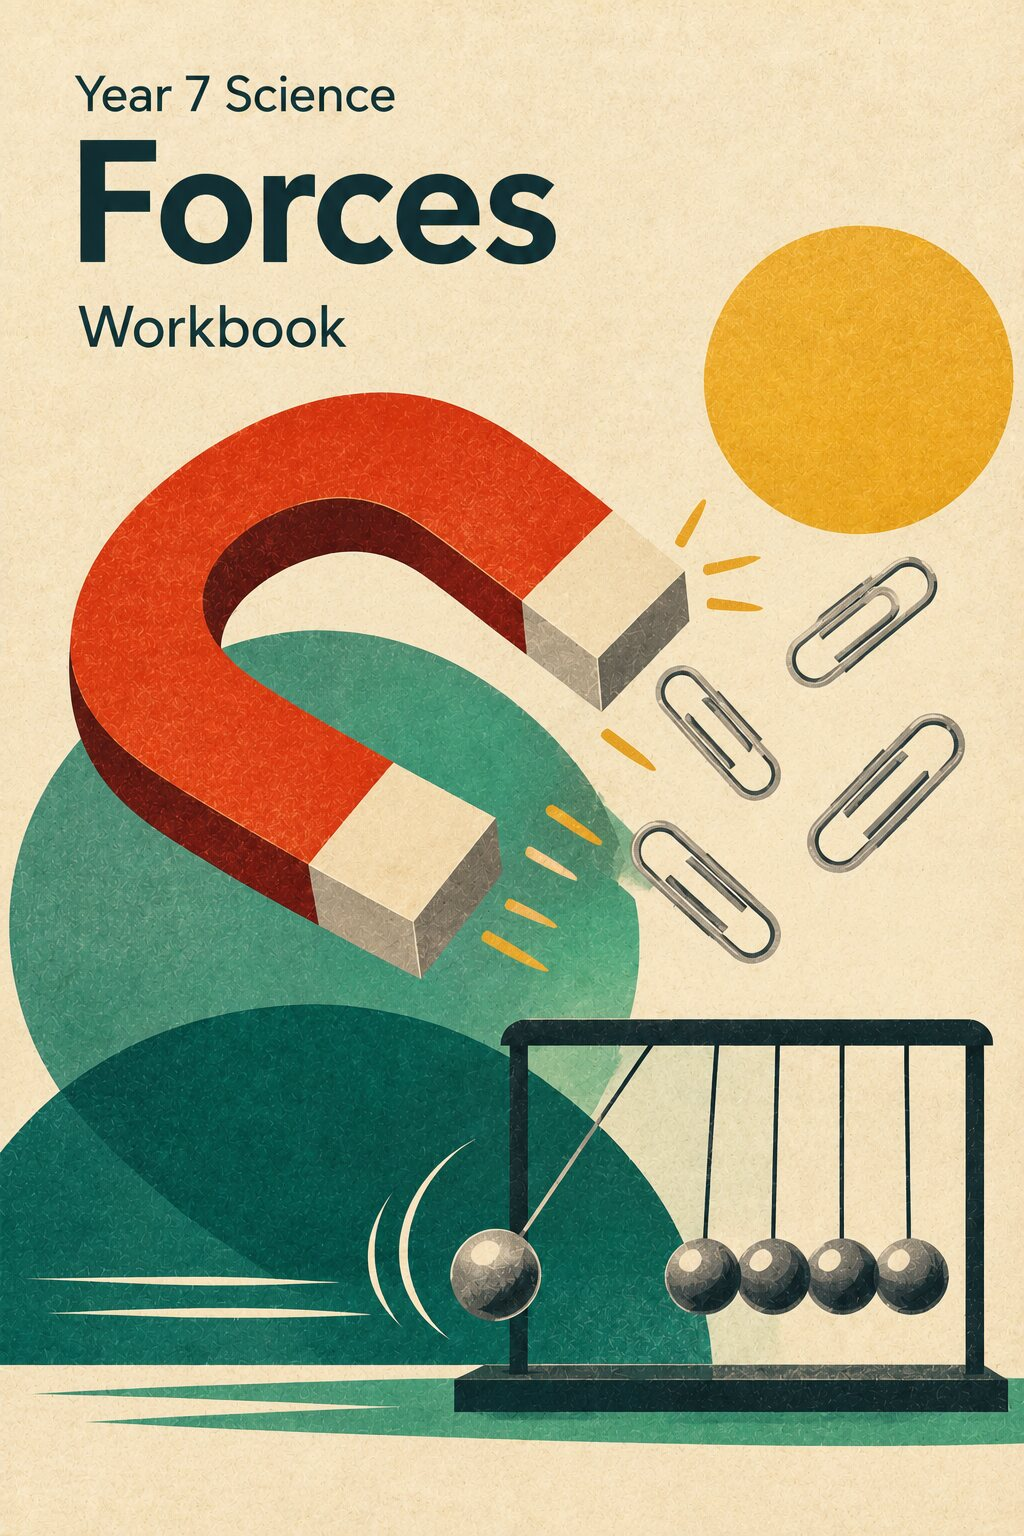
\includegraphics[width=\paperwidth]{../../../covers/forces.jpg}};
  \node[anchor=north east, fill=white, draw=Ink, line width=0.6pt, rounded corners=1.2mm,
        inner xsep=2mm, inner ysep=1.8mm, text width=30mm, font=\headingfont\footnotesize]
    at ([xshift=-4mm, yshift=-4mm]current page.north east)
    {\textbf{Name}\par\vspace{4mm}\hrule\vspace{2mm}\textbf{Class}\par\vspace{4mm}\hrule};
  \node[anchor=south east, fill=white, draw=Ink, line width=0.6pt, rounded corners=1.2mm,
        inner xsep=2.6mm, inner ysep=2mm, font=\headingfont\bfseries, align=right]
    at ([xshift=-4mm, yshift=6mm]current page.south east)
    {Lesson Booklet 2\\[-1pt]{\normalfont\headingfont\scriptsize Lessons 5--9}};
\end{tikzpicture}
\mbox{}
\clearpage

% ---- Inside cover ---------------------------------------------------------
\thispagestyle{plain}
{\headingfont\bfseries\fontsize{22}{26}\selectfont Forces and Motion}\par\vspace{1mm}
{\headingfont\large Lesson Booklet 2 \textbullet\ Lessons 5--9 \textbullet\ Year 7}\par\vspace{1mm}
{\small\itshape VC 2.0: VC2S8U13 \textbullet\ VC2S8U14 \textbullet\ VC2S8U15 \textbullet\ VC2S8I01--I08}\par\vspace{4mm}
\textbf{Teacher}\ \hrulefill\par

\begin{countrybox}{Acknowledgement of Country}
This booklet was created on the unceded Country of the Wurundjeri Woi-wurrung people of the Kulin Nation. We acknowledge Elders past, present and emerging.
\end{countrybox}

\begin{infobox}{How this booklet works}
One section for each lesson. Each opens with its key vocabulary, then:\par\smallskip
\renewcommand{\arraystretch}{1.25}
\begin{tabular}{@{}p{24mm}p{70mm}@{}}
\textbf{Part A} & a reading with comprehension questions \\
\textbf{Part B} & the ideas, worked through \\
\textbf{Part C} & practice on your own \\
\textbf{Part D} & above level: Year 8 extension \\
\end{tabular}

\smallskip
\begin{tabular}{@{}p{24mm}p{70mm}@{}}
\textbf{I do} \tagicon{\icodots{1}} & your teacher works an example (solid frame) \\
\textbf{We do} \tagicon{\icodots{2}} & you try one together (dashed frame) \\
\textbf{Reading} \tagicon{\icoread} & a passage to read (thin frame) \\
\textbf{Above level} \tagicon{\icoup} & extension (double frame) \\
\end{tabular}

\smallskip
Three lesson books. The five experiments are in the \textbf{Experiment Booklet}; the trebuchet investigation has its own booklet.
\end{infobox}

\clearpage
\markboth{Contents}{Contents}
{\headingfont\bfseries\LARGE Contents}\par\vspace{1mm}\noindent\rule{\linewidth}{0.6pt}\par\vspace{2mm}
\renewcommand{\arraystretch}{1.12}
\begin{tabular}{|C{1.1cm}|L{6.0cm}|C{2.4cm}|}
  \hline\thead{Lesson} & \thead{Title} & \thead{Page} \\ \hline
  1 & What is a Force? & Book 1 \\ \hline
  2 & Force Diagrams and Net Force & Book 1 \\ \hline
  3 & \textit{Experiment 1 --- Everyday Forces} & {\footnotesize Experiment Booklet} \\ \hline
  4 & Newton's First and Third Laws & Book 1 \\ \hline
  5 & \hyperlink{lesson.5.1}{Newton's Second Law: \texorpdfstring{$F = ma$}{F = ma}} & \hyperlink{lesson.5.1}{p.\ \pageref{sec:5}} \\ \hline
  6 & \textit{Experiment 2 --- Friction and Mass} & {\footnotesize Experiment Booklet} \\ \hline
  7 & \hyperlink{lesson.7.1}{Energy and Transformation} & \hyperlink{lesson.7.1}{p.\ \pageref{sec:7}} \\ \hline
  8 & \textit{Experiment 3 --- Bounce Efficiency} & {\footnotesize Experiment Booklet} \\ \hline
  9 & \hyperlink{lesson.9.1}{Simple Machines and Levers} & \hyperlink{lesson.9.1}{p.\ \pageref{sec:9}} \\ \hline
  10 & \textit{Experiment 4 --- Lever Mechanical Advantage} & {\footnotesize Experiment Booklet} \\ \hline
  11 & Levers Extension (Optional) & Book 3 \\ \hline
  12 & Projectile Motion & Book 3 \\ \hline
  13 & \textit{Experiment 5 --- Measuring $g$} & {\footnotesize Experiment Booklet} \\ \hline
  14 & Optimising Range (Optional) & Book 3 \\ \hline
  15 & \textit{Trebuchet investigation: planning} & {\footnotesize Trebuchet booklet} \\ \hline
  16 & \textit{Trebuchet investigation: launches} & {\footnotesize Trebuchet booklet} \\ \hline
  17 & \textit{Trebuchet investigation: analysis and conclusion} & {\footnotesize Trebuchet booklet} \\ \hline
  --- & \hyperlink{glossary}{Glossary} & \hyperlink{glossary}{\pageref{sec:glossary}} \\ \hline
\end{tabular}
\renewcommand{\arraystretch}{1}
\clearpage
\setcounter{section}{4}\renewcommand{\lessonart}{5}
% ══════════════════════════════════════════════════════════════════════════════
%  LESSON 5 — NEWTON'S SECOND LAW                                 (Week 2 · P2)
% ══════════════════════════════════════════════════════════════════════════════
\sectiondiv{Newton's Second Law: \texorpdfstring{$F = ma$}{F = ma}}{Acceleration \textbullet{} Force, mass and acceleration \textbullet{} Rearranging $F = ma$ \textbullet{} Using the net force}\label{sec:5}
\lessoncodes{VC2S8U14 \textbullet{} VC2S10U17 (above level)}

\vocabhead
\begin{ctab}
\begin{tabular}{|SW{2.91cm}|W{8.05cm}|}
  \hd & \thead{Word} & \thead{Definition (copy from the slide)} \\ \hline
  & \scaf{\textbf{Acceleration}\label{voc:acceleration}} & \scaf{How quickly an object's speed changes, measured in metres per second squared ($\text{m/s}^2$).} \\ \hline
  & \textbf{Deceleration}\label{voc:deceleration} & \cell{5.v2} \\ \hline
  & \textbf{Newton's Second Law}\label{voc:newton-s-second-law} & \cell{5.v3} \\ \hline
  & \textbf{Directly proportional}\label{voc:directly-proportional} & \cell{5.v4} \\ \hline
  & \textbf{Rearrange}\label{voc:rearrange} & \cell{5.v5} \\ \hline
\end{tabular}
\end{ctab}

% ─── PART A ───────────────────────────────────────────────────────────────────
\lessonpart{A}{Reading and comprehension}{Teal}\label{read:5}

\begin{readingbox}{Reading --- Pushing a Broken-Down Car}
A car has broken down on a quiet, flat street, and it needs to be pushed to the side of the road. One person leans against the back and pushes as hard as they can. Slowly --- very slowly --- the car starts to roll. Two friends run over to help, and with three people pushing, the car speeds up much more quickly. A bigger force gives a bigger acceleration.

Further down the street, a removalist's van packed full of furniture has also broken down. The same three people push it just as hard as they pushed the car. This time it barely creeps forwards. The force is the same, but the van has far more mass, and more mass means a smaller acceleration.

Once the car is rolling, something changes: the pushers can ease off. They only need to push hard enough to match the friction acting on the car, and it keeps rolling at a steady speed. Pushing harder only matters if they want it to go faster.

Isaac Newton tied all of this together in his Second Law: how quickly an object speeds up depends on the net force acting on it, and on its mass. That is why racing cars and racing bikes are built to be as light as possible. With the same engine, or the same legs, a lighter vehicle speeds up faster.
\end{readingbox}

\rcreset
\rcqk{5.c1}{What happened to the car's acceleration when two friends joined in? Explain why.}{1.6cm}
\rcqk{5.c2}{The same push was used on the loaded van. Describe what happened, and explain it using the word \emph{mass}.}{1.8cm}
\rcqk{5.c3}{Once the car rolls at a steady speed, which force are the pushers balancing? How do you know the forces are balanced?}{1.8cm}
\rcqk{5.c4}{Why are racing cars and racing bikes built to be as light as possible?}{1.6cm}
\rcqk{5.c5}{According to the passage, what \emph{two} things decide how quickly an object speeds up?}{1.4cm}
\rcqk{5.c6}{Which sentence in the first paragraph sums up what happened when more people pushed the car?}{1.4cm}
\rcqk{5.c7}{Describe one other everyday example where the same push gives a smaller acceleration because the object has more mass.}{1.6cm}
\rcqk{5.c8}{Suppose the three pushers kept pushing just as hard after the car was already rolling. Using the passage, predict what would happen to the car, and explain why using the words \emph{net force}.}{2.0cm}

% ─── PART B ───────────────────────────────────────────────────────────────────
\lessonpart{B}{Theory and examples}{Blue}\label{theory:5}

\subsection{What is Acceleration?}\label{sub:5.1}

\textbf{Acceleration} is how quickly an object's speed changes. It is measured in \textbf{metres per second squared (m/s$^2$)}, which means ``metres per second, every second''.

\begin{infobox}{Reading an acceleration}
An acceleration of \textbf{3\,m/s$^2$} means the speed goes up by \textbf{3\,m/s every second}. Starting from rest:

\medskip
\begin{tabular}{|l|c|c|c|c|}
  \hline
  \textbf{Time (s)}    & 0 & 1 & 2 & 3 \\ \hline
  \textbf{Speed (m/s)} & 0 & 3 & 6 & 9 \\ \hline
\end{tabular}

\medskip
Slowing down is also an acceleration. It is sometimes called a \textbf{deceleration}.
\end{infobox}

\subsection{Force, Mass and Acceleration}\label{sub:5.2}

Newton's Second Law links three things: the \textbf{net force} on an object, its \textbf{mass}, and its \textbf{acceleration}.

\diagFma
\figcap[fig:fma]{Newton's Second Law: force, mass and acceleration}

\vspace{2pt}
\begin{ctab}
\begin{tabular}{|L{3.79cm}|L{2.25cm}|L{4.50cm}|}
  \thead{If you\ldots} & \thead{the acceleration\ldots} & \thead{Example} \\ \hline
  \talt increase the force (same mass) & increases & Three people push the car instead of one \\ \hline
        increase the mass (same force) & decreases & The same push on a loaded van \\ \hline
  \talt double the force (same mass)   & doubles   & Two people push a trolley, each as hard as one did before \\ \hline
        double the mass (same force)   & halves    & The same push on two identical trolleys joined together \\ \hline
\end{tabular}
\end{ctab}

\needspace{11\baselineskip}
\begin{infobox}{Second Law}
The acceleration of an object is directly proportional to the net force acting on it, and inversely proportional to its mass.
\[
  \boxed{F = m \times a}
  \qquad\qquad
  \boxed{a = \frac{F}{m}}
  \qquad\qquad
  \boxed{m = \frac{F}{a}}
\]
Force in newtons (N) \quad Mass in kilograms (kg) \quad Acceleration in m/s$^2$
\end{infobox}
\newpage
\subsection{Using $F = ma$}\label{sub:5.3}

You only need to remember one formula. The \textbf{formula triangle} shows how to rearrange it.

\diagFmaTriangle
\figcap{The formula triangle. Cover the quantity you want; what is left shows how to find it.}

\begin{skillbox}{Four steps for every $F = ma$ question}
\begin{enumerate}[itemsep=1pt, leftmargin=1.4em, topsep=1pt]
  \item Write down what you \textbf{know}, with units.
  \item Choose the \textbf{version} of the formula you need (use the triangle).
  \item \textbf{Substitute} the numbers.
  \item \textbf{Calculate}, and always write the \textbf{unit}.
\end{enumerate}
\end{skillbox}

\begin{workedex}{Finding acceleration}
A 5\,kg trolley is pushed with a net force of 20\,N. What is its acceleration?

\medskip
\textbf{Know:}\quad $F = 20$\,N, \quad $m = 5$\,kg

\textbf{Formula:}\quad $F = m \times a$ \quad $\Rightarrow$ \quad $a = F \div m$

\textbf{Substitute:}\quad $a = 20 \div 5 = \mathbf{4\ \text{m/s}^2}$
\end{workedex}

\begin{wedo}{Finding acceleration}
A 3\,kg toy car is pushed with a net force of 15\,N. What is its acceleration?
\wbox{5.wd1}{2.8cm}
\end{wedo}

\begin{workedex}{Finding force}
A 1200\,kg car accelerates at 2\,m/s$^2$. What net force is acting on it?

\medskip
\textbf{Know:}\quad $m = 1200$\,kg, \quad $a = 2$\,m/s$^2$

\textbf{Formula:}\quad $F = m \times a$

\textbf{Substitute:}\quad $F = 1200 \times 2 = \mathbf{2400\ \text{N}}$
\end{workedex}

\begin{wedo}{Finding force}
A 0.5\,kg ball accelerates at 12\,m/s$^2$ when it is thrown. What net force acts on it?
\wbox{5.wd2}{2.8cm}
\end{wedo}

\begin{workedex}{Finding mass}
A net force of 60\,N gives a box an acceleration of 4\,m/s$^2$. What is the mass of the box?

\medskip
\textbf{Know:}\quad $F = 60$\,N, \quad $a = 4$\,m/s$^2$

\textbf{Formula:}\quad $F = m \times a$ \quad $\Rightarrow$ \quad $m = F \div a$

\textbf{Substitute:}\quad $m = 60 \div 4 = \mathbf{15\ \text{kg}}$
\end{workedex}

\begin{wedo}{Finding mass}
A net force of 80\,N gives a wheelbarrow an acceleration of 5\,m/s$^2$. What is the mass of the wheelbarrow?
\wbox{5.wd3}{2.8cm}
\end{wedo}

\subsection{Always Use the Net Force}\label{sub:5.4}

The $F$ in $F = ma$ is the \textbf{net force} --- the force left over after you add up all the forces (Lesson~2). If the forces are balanced, the net force is zero, so the acceleration is zero: the object stays still, or keeps moving at a steady speed. That is exactly what the First Law says.

\begin{workedex}{Net force first}
A 10\,kg trolley is pushed forwards with 50\,N. Friction pushes back with 10\,N. Find its acceleration.

\medskip
\textbf{Step 1 --- net force:}\quad opposite directions, so subtract: \quad $50 - 10 = 40$\,N forwards

\textbf{Step 2 --- acceleration:}\quad $a = F \div m = 40 \div 10 = \mathbf{4\ \text{m/s}^2}$ \textbf{forwards}
\end{workedex}

\begin{wedo}{Net force first}
A 25\,kg go-kart is pushed forwards with 120\,N. Friction pushes back with 45\,N.
\pt{a}Find the net force.
\wbox{5.wd4a}{1.8cm}
\pt{b}Find the acceleration of the go-kart.
\wbox{5.wd4b}{1.8cm}
\end{wedo}

% ─── PART C ───────────────────────────────────────────────────────────────────
\lessonpart{C}{Practice}{Amber}\label{prac:5}

Work through every task. Show your working for calculations, and always include the unit.

\needspace{12\baselineskip}
\task For each change, describe what happens to the acceleration. Write \textbf{increases}, \textbf{decreases}, \textbf{doubles} or \textbf{halves}.

\vspace{4pt}
\begin{ctab}
\begin{tabular}{|SW{3.51cm}|Z{1.55cm}|W{3.51cm}|Z{1.55cm}|}
  \hd & \thead{Change} & \thead{\scriptsize Acceleration} & \thead{Change} & \thead{\scriptsize Acceleration} \\ \hline
  & The force is doubled; the mass stays the same & \scaf{doubles} & The mass is doubled; the force stays the same & \scaf{halves} \\ \hline
  & More people help push the same car & \cell{5.t1-r2c2} & A heavier rider pedals the same bike just as hard & \cell{5.t1-r2c4} \\ \hline
  & A truck is loaded with bricks; its engine force stays the same & \cell{5.t1-r3c2} & A rocket burns fuel and gets lighter; its thrust stays the same & \cell{5.t1-r3c4} \\ \hline
\end{tabular}
\end{ctab}

\needspace{12\baselineskip}
\task Use $F = ma$ to complete the table. The first row is done for you.

\vspace{4pt}
\begin{ctab}
\begin{tabular}{|SW{3.09cm}|Z{2.25cm}|Z{2.25cm}|Z{2.53cm}|}
  \hd & \thead{Situation} & \thead{Force (N)} & \thead{Mass (kg)} & \thead{Acceleration (m/s$^2$)} \\ \hline
  & Trolley pushed      & 20     & 5    & \scaf{$a = 20 \div 5 = 4$} \\ \hline
  & Soccer ball kicked  & 45     & 0.45 & \cell{5.t2-r2c4} \\ \hline
  & Car braking         & \cell{5.t2-r3c2} & 1200 & 3.5 \\ \hline
  & Rocket launch       & 6\,000 & \cell{5.t2-r4c3} & 30 \\ \hline
\end{tabular}
\end{ctab}

\taskpair{A net force of 24\,N acts on a 6\,kg mass. Find the acceleration.}{\wbox{5.t3}{2.4cm}}
         {A 0.5\,kg ball accelerates at 12\,m/s$^2$. Find the net force.}{\wbox{5.t4}{2.4cm}}

\taskpair{A force of 90\,N gives an object an acceleration of 3\,m/s$^2$. Find its mass.}{\wbox{5.t5}{2.4cm}}
         {A 1500\,kg car accelerates at 2.5\,m/s$^2$. Find the net force needed.}{\wbox{5.t6}{2.4cm}}

\taskpair{A 70\,kg sprinter accelerates at 4\,m/s$^2$ out of the blocks. Find the net force on her.}{\wbox{5.t7}{2.4cm}}
         {A 0.15\,kg cricket ball is hit with a net force of 30\,N. Find its acceleration.}{\wbox{5.t8}{2.4cm}}

\needspace{14\baselineskip}
\task A 2.5\,kg trolley is pushed with different net forces.
\pt{a}Complete the table.

\vspace{4pt}
\begin{ctab}
\begin{tabular}{|SZ{2.89cm}|Z{2.89cm}|Z{4.76cm}|}
  \hd & \thead{Net force (N)} & \thead{Mass (kg)} & \thead{Acceleration (m/s$^2$)} \\ \hline
  & 5  & 2.5 & \scaf{$a = 5 \div 2.5 = 2$} \\ \hline
  & 10 & 2.5 & \cell{5.t9a-r2c3} \\ \hline
  & 15 & 2.5 & \cell{5.t9a-r3c3} \\ \hline
  & 20 & 2.5 & \cell{5.t9a-r4c3} \\ \hline
\end{tabular}
\end{ctab}
\pt{b}What happens to the acceleration each time the force goes up by 5\,N? Describe the pattern.
\abox{5.t9b}{2.0cm}

\needspace{10\baselineskip}
\task A shopping trolley of mass 15\,kg is pushed with a force of 45\,N. Friction opposes the motion with 15\,N.
\pt{a}Find the net force.
\wbox{5.t10a}{2.0cm}
\pt{b}Find the acceleration of the trolley.
\wbox{5.t10b}{2.0cm}

\needspace{10\baselineskip}
\task A 60\,kg cyclist and her 12\,kg bicycle accelerate at 1.5\,m/s$^2$.
\pt{a}Find the total mass.
\wbox{5.t11a}{2.0cm}
\pt{b}Find the net force.
\wbox{5.t11b}{2.0cm}
\pt{c}Air resistance is 30\,N. Find the force she must produce by pedalling.
\wbox{5.t11c}{2.0cm}

\needspace{10\baselineskip}
\task Two identical trolleys are pushed with the same force. Trolley A is empty, with a mass of 2\,kg. Trolley B carries an extra 6\,kg, so its total mass is 8\,kg.
\pt{a}Which trolley accelerates more?
\abox{5.t12a}{2.0cm}
\pt{b}Explain your answer using $F = ma$.
\abox{5.t12b}{2.0cm}
\pt{c}The force is 16\,N. Calculate both accelerations.
\wbox{5.t12c}{2.0cm}

\needspace{10\baselineskip}
\task A net force of 3600\,N gives a car an acceleration of 2\,m/s$^2$.
\pt{a}Find the mass of the car.
\wbox{5.t13a}{2.0cm}
\pt{b}The car is then loaded with 200\,kg of luggage. Find its new acceleration with the same net force.
\wbox{5.t13b}{2.0cm}

\needspace{10\baselineskip}
\task A 900\,kg car travels along a flat road at a steady 60\,km/h. Its engine provides a driving force of 2000\,N.
\pt{a}What is the car's acceleration? Explain how you know.
\abox{5.t14a}{2.0cm}
\pt{b}What is the total size of the resistive forces (friction and air resistance) acting on the car?
\abox{5.t14b}{2.0cm}

% ─── PART D ───────────────────────────────────────────────────────────────────
\lessonpart{D}{Above level}{Violet}\label{ext:5}

\begin{yr8box}
These questions go beyond the Year 7 standard. They ask you to combine ideas, use more than one formula, or judge someone else's reasoning.

\medskip
\needspace{10\baselineskip}
\exttask Ahmed pushes a 20\,kg crate with a force of 60\,N, but it does not move. He says: \emph{``$F = ma$ means it should accelerate at 3\,m/s$^2$, so the formula must be wrong.''} Explain Ahmed's mistake, and find the size of the friction force on the crate.
\wbox{5.x15}{3.0cm}

\needspace{10\baselineskip}
\exttask Mia pushes a 50\,kg crate across the floor. Friction on the crate is 40\,N. She says: \emph{``If I push twice as hard, the crate will speed up twice as fast.''}
\pt{a}Find the acceleration when she pushes with 100\,N.
\wbox{5.x16a}{2.0cm}
\pt{b}Find the acceleration when she pushes with 200\,N.
\wbox{5.x16b}{2.0cm}
\pt{c}Is Mia right? Explain, using the idea of net force.
\abox{5.x16c}{2.0cm}

\needspace{10\baselineskip}
\exttask A rocket's engines push exhaust gas downwards with a force of 500\,000\,N, and the gas pushes the rocket upwards with the same force. The rocket has a mass of 20\,000\,kg. Use $g = 9.8$\,N/kg.
\pt{a}Find the rocket's weight.
\wbox{5.x17a}{2.0cm}
\pt{b}Find the net force on the rocket at lift-off.
\wbox{5.x17b}{2.0cm}
\pt{c}Find its acceleration.
\wbox{5.x17c}{2.0cm}
\pt{d}Which of Newton's laws explains (i) the upward push of the gas, and (ii) the size of the acceleration?
\abox{5.x17d}{2.0cm}

\needspace{10\baselineskip}
\exttask A lift and its passengers have a total mass of 800\,kg. The cable pulls the lift upwards with a force of 8640\,N. Use $g = 9.8$\,N/kg.
\pt{a}Find the weight of the lift and its passengers.
\wbox{5.x18a}{2.0cm}
\pt{b}Find the size and direction of the net force.
\wbox{5.x18b}{2.0cm}
\pt{c}Find the acceleration of the lift.
\wbox{5.x18c}{2.0cm}

\needspace{10\baselineskip}
\exttask A cyclist speeds up from 2\,m/s to 8\,m/s in 4\,s. The cyclist and bicycle have a total mass of 80\,kg.
\pt{a}Calculate the acceleration, using $a = \Delta v \div t$ (change in speed $\div$ time).
\wbox{5.x19a}{2.0cm}
\pt{b}Calculate the net force on the cyclist and bicycle.
\wbox{5.x19b}{2.0cm}
\pt{c}Air resistance and friction total 40\,N. Find the force the cyclist must supply by pedalling.
\wbox{5.x19c}{2.0cm}

\needspace{10\baselineskip}
\exttask A 0.045\,kg golf ball is struck and leaves the tee at 60\,m/s. The club is in contact with the ball for 0.0005\,s.
\pt{a}Calculate the acceleration of the ball, using $a = \Delta v \div t$ (change in speed $\div$ time).
\wbox{5.x20a}{2.0cm}
\pt{b}Calculate the force applied by the club.
\wbox{5.x20b}{2.0cm}
\pt{c}Calculate the ball's weight, and comment on how the force from the club compares with it.
\wbox{5.x20c}{2.0cm}

\needspace{10\baselineskip}
\exttask In the trebuchet investigation at the end of this unit, a sling swings a 0.05\,kg projectile. While it is being swung, the net force on the projectile is 2\,N.
\pt{a}Find the projectile's acceleration.
\wbox{5.x21a}{2.0cm}
\pt{b}The sling pulls on the projectile. Describe the reaction force.
\abox{5.x21b}{2.0cm}
\pt{c}Once the projectile leaves the sling, nothing pushes it forwards. Explain why it keeps moving forwards, and name the force that brings it back to the ground.
\abox{5.x21c}{2.0cm}
\end{yr8box}

\newpage
\setcounter{section}{6}\renewcommand{\lessonart}{7}
% ══════════════════════════════════════════════════════════════════════════════
%  LESSON 7 — ENERGY AND TRANSFORMATION                           (Week 3 · P1)
% ══════════════════════════════════════════════════════════════════════════════
\sectiondiv{Energy and Transformation}{Forms of energy \textbullet{} Energy chains \textbullet{} Conservation and efficiency \textbullet{} GPE and KE}\label{sec:7}
\lessoncodes{VC2S8U15 \textbullet{} VC2S10U15 (above level)}

\vocabhead
\begin{ctab}
\begin{tabular}{|SW{2.91cm}|W{8.05cm}|}
  \hd & \thead{Word} & \thead{Definition (copy from the slide)} \\ \hline
  & \scaf{\textbf{Energy}\label{voc:energy}} & \scaf{The ability to make something happen. It is measured in joules (J).} \\ \hline
  & \textbf{Kinetic energy}\label{voc:kinetic-energy} & \cell{7.v2} \\ \hline
  & \textbf{Gravitational potential energy}\label{voc:gravitational-potential-energy} & \cell{7.v3} \\ \hline
  & \textbf{Energy transformation}\label{voc:energy-transformation} & \cell{7.v4} \\ \hline
  & \textbf{Conservation of energy}\label{voc:conservation-of-energy} & \cell{7.v5} \\ \hline
  & \textbf{Efficiency}\label{voc:efficiency} & \cell{7.v6} \\ \hline
\end{tabular}
\end{ctab}

% ─── PART A ───────────────────────────────────────────────────────────────────
\vspace*{-10pt}% tighter gap above Part A so the whole reading fits on this page
\lessonpart{A}{Reading and comprehension}{Teal}\label{read:7}

\begin{readingbox}{Reading --- Why the First Hill is Always the Tallest}
\small % one size down so the whole reading fits on the lesson's first page
Look carefully at a traditional roller coaster --- the kind that is pulled up its first hill by a chain --- and you will notice something: the first hill is always the highest one on the track. This is not a matter of taste or thrill design. It is a rule imposed by physics, and no engineer can get around it.

The train itself has no engine. A chain drags it slowly up that first hill, and after that the ride is entirely powered by gravity. Hauling the train to the top stores energy in it --- gravitational potential energy --- and the amount stored depends on how high the train is lifted. As the train plunges down, that stored energy is converted into kinetic energy, the energy of movement, and the train reaches its greatest speed at the bottom. Climbing the next hill converts kinetic energy back into potential energy, and so the ride continues, trading one form for the other.

The catch is that the swap is never perfect. Every time the wheels turn, a little energy is lost as heat through friction, and a little more is lost as sound --- that familiar roar. Because energy cannot be created, the train can never climb higher than it started. Each successive hill must be a little lower than the one before, and the ride must end before the energy runs out entirely.

At the end of the ride the train still has some kinetic energy, and it has to be removed safely. Many modern coasters use magnetic brakes: metal fins under the train pass between strong magnets, and the magnets slow the fins down without ever touching them. The train's kinetic energy is not destroyed --- it ends up as thermal energy, warming the fins and the air around them.
\end{readingbox}

\rcreset
\rcqk{7.c1}{Where does a roller coaster train get the energy for the whole ride, and how is that energy stored?}{1.8cm}
\rcqk{7.c2}{Describe the energy transformation that happens as the train travels down the first hill.}{1.8cm}
\rcqk{7.c3}{Explain why each hill on the track must be lower than the one before it. Name the two ways energy is lost.}{2.0cm}
\rcqk{7.c4}{At which point on the ride does the train have the most kinetic energy? Explain how you know.}{1.6cm}
\rcqk{7.c5}{Which phrase in the third paragraph tells you that energy cannot simply appear from nowhere?}{1.4cm}
\rcqk{7.c6}{How do magnetic brakes stop the train, and what happens to the train's kinetic energy?}{1.8cm}
\rcqk{7.c7}{In your own words, explain what the passage means when it says the swap between potential and kinetic energy is ``never perfect''.}{1.8cm}

% ─── PART B ───────────────────────────────────────────────────────────────────
\lessonpart{B}{Theory and examples}{Blue}\label{theory:7}

\subsection{Forms of Energy}\label{sub:7.1}

\textbf{Energy} is what makes things happen: it is needed to move something, heat it, light it up or make a sound. Energy is measured in \textbf{joules (J)}. It comes in several forms. Some are \emph{stored} energy, waiting to be used; others show that something is \emph{happening}.

\vspace{4pt}
\begin{ctab}
\begin{tabular}{|L{2.95cm}|L{3.93cm}|L{3.65cm}|}
  \thead{Form of energy} & \thead{What it is} & \thead{Example} \\ \hline
  \talt Kinetic              & The energy of anything that is moving & A rolling ball, a moving car \\ \hline
        Gravitational potential & Energy stored by lifting something up high & A book on a high shelf \\ \hline
  \talt Elastic potential    & Energy stored by stretching or squashing & A stretched rubber band \\ \hline
        Chemical             & Energy stored in food, fuel and batteries & A sandwich, petrol, a battery \\ \hline
  \talt Thermal              & Energy of hot objects; hotter means more & A cup of hot tea \\ \hline
        Sound, light and electrical & Energy carried by sound waves, light and electric current & A speaker, a torch beam, a power cable \\ \hline
\end{tabular}
\end{ctab}

\diagEnergy
\figcap[fig:energy-types]{Three forms of energy you will meet again and again, and how energy changes form in a trebuchet}

\vspace*{-2mm}% a touch less space above 7.2 so Worked Example 7.1 stays whole on its page
\subsection{Transformations and Energy Chains}\label{sub:7.2}

Energy can change from one form to another. This is called an \textbf{energy transformation}. An \textbf{energy chain} shows each step, with an arrow for every change. The trebuchet in Figure~\ref{fig:energy-types} turns the gravitational potential energy of its raised counterweight into kinetic energy of the arm, and then of the ball.

\begin{workedex}{An energy chain for a bouncing ball}
A ball is held above the floor, dropped, and bounces back up. Write the energy chain from the moment it is let go to the top of its bounce.

\medskip
\textbf{Falling:} gravitational potential $\rightarrow$ kinetic \quad(it speeds up as it falls)

\textbf{Hitting the floor:} kinetic $\rightarrow$ elastic potential \quad(the ball squashes)

\textbf{Bouncing up:} elastic potential $\rightarrow$ kinetic $\rightarrow$ gravitational potential

\medskip
At every step a little energy is \textbf{wasted} as thermal energy and sound --- you can hear the bounce.
\end{workedex}

\begin{wedo}{An energy chain for a skateboarder}
A skateboarder starts at rest at the top of a half-pipe ramp, rolls down, and rolls up the other side.
\pt{a}Write the energy chain from the top of the ramp to the top of the other side.
\abox{7.wd1a}{2.0cm}
\pt{b}Explain why the skateboarder does not quite reach the same height on the other side.
\abox{7.wd1b}{2.0cm}
\end{wedo}

\subsection{Conservation of Energy and Efficiency}\label{sub:7.3}

\begin{infobox}{The Law of Conservation of Energy}
Energy \textbf{cannot be created or destroyed}. It can only be transformed from one form to another, or transferred from one object to another. The total amount of energy at the end is always the same as at the start.
\end{infobox}

So where does energy ``go''? Not all of it ends up where we want it. The energy that does the job we want is \textbf{useful} energy. The rest is \textbf{wasted} energy --- usually thermal energy and sound, which spread out into the surroundings and are hard to use again. A \textbf{Sankey diagram} shows this with arrows whose width matches the amount of energy.

\diagSankey
\figcap[fig:sankey]{A Sankey diagram. The useful and wasted arrows always add up to the energy in.}

\begin{infobox}{Efficiency}
\[ \text{Efficiency} = \frac{\text{useful energy out}}{\text{total energy in}} \times 100\% \]
A machine that wastes no energy would be 100\% efficient. No real machine is.
\end{infobox}

\begin{workedex}{Calculating efficiency}
An old-style light bulb is supplied with 100\,J of electrical energy. It gives out 5\,J of light. How much energy is wasted, and what is its efficiency?

\medskip
\textbf{Wasted:}\quad $100 - 5 = \mathbf{95\ \text{J}}$ \quad (as thermal energy --- the bulb gets hot)

\textbf{Efficiency:}\quad $5 \div 100 \times 100\% = \mathbf{5\%}$
\end{workedex}

\begin{wedo}{Calculating efficiency}
An LED globe is supplied with 100\,J of electrical energy. It gives out 40\,J of light.
\pt{a}How much energy is wasted?
\wbox{7.wd2a}{1.6cm}
\pt{b}What is its efficiency?
\wbox{7.wd2b}{1.8cm}
\end{wedo}

\subsection{Calculating Gravitational Potential and Kinetic Energy}\label{sub:7.4}

\begin{infobox}{Two energy formulas}
\[ \text{GPE} = m \times g \times h \qquad\qquad \text{KE} = \tfrac{1}{2} \times m \times v^2 \]
$m$ = mass (kg) \quad $g = 9.8$\,N/kg on Earth \quad $h$ = height (m) \quad $v$ = speed (m/s) \quad Energy in joules (J)
\end{infobox}

\begin{workedex}{Gravitational potential energy}
A 2\,kg ball is held at a height of 5\,m. Find its gravitational potential energy.

\medskip
$\text{GPE} = mgh = 2 \times 9.8 \times 5 = \mathbf{98\ \text{J}}$
\end{workedex}

\begin{wedo}{Gravitational potential energy}
A 5\,kg box is lifted onto a shelf 1.5\,m high. Find its gravitational potential energy. Use $g = 9.8$\,N/kg.
\wbox{7.wd3}{2.4cm}
\end{wedo}

\begin{workedex}{Kinetic energy}
A 4\,kg dog runs at 3\,m/s. Find its kinetic energy.

\medskip
\textbf{Square the speed first:}\quad $v^2 = 3 \times 3 = 9$

\textbf{Then:}\quad $\text{KE} = \tfrac{1}{2} \times m \times v^2 = 0.5 \times 4 \times 9 = \mathbf{18\ \text{J}}$
\end{workedex}

\begin{wedo}{Kinetic energy}
A 6\,kg bowling ball rolls at 2\,m/s. Find its kinetic energy.
\wbox{7.wd4}{2.4cm}
\end{wedo}

When the 2\,kg ball in Worked Example~\ref{we:7.3} is dropped, its 98\,J of gravitational potential energy becomes kinetic energy. Just before it lands it has close to 98\,J of kinetic energy --- a little less, because some is wasted pushing through the air.

% ─── PART C ───────────────────────────────────────────────────────────────────
\lessonpart{C}{Practice}{Amber}\label{prac:7}

Work through every task. Use $g = 9.8$\,N/kg. Show your working for calculations, and always include the unit.

\needspace{12\baselineskip}
\task For each object, name the main form of energy it has. Write it in the box.

\vspace{4pt}
\begin{ctab}
\begin{tabular}{|SW{3.46cm}|Z{1.73cm}|W{3.20cm}|Z{1.73cm}|}
  \hd & \thead{Object} & \thead{Form of energy} & \thead{Object} & \thead{Form of energy} \\ \hline
  & A stretched rubber band & \scaf{elastic potential} & A bowling ball rolling down the lane & \scaf{kinetic} \\ \hline
  & A rock balanced on a cliff edge & \cell{7.t1-r2c2} & A battery & \cell{7.t1-r2c4} \\ \hline
  & A cup of hot chocolate & \cell{7.t1-r3c2} & A drawn-back bowstring & \cell{7.t1-r3c4} \\ \hline
  & A sandwich & \cell{7.t1-r4c2} & A child sliding down a slide & \cell{7.t1-r4c4} \\ \hline
\end{tabular}
\end{ctab}

\needspace{14\baselineskip}
\task Complete the table. For each device, name the form of energy that goes in, the useful energy that comes out, and the main wasted energy.

\vspace{4pt}
\begin{ctab}
\begin{tabular}{|SW{2.36cm}|Z{2.50cm}|Z{2.63cm}|Z{2.63cm}|}
  \hd & \thead{Device} & \thead{Energy in} & \thead{Useful energy out} & \thead{Wasted energy} \\ \hline
  & Torch & \scaf{chemical (battery)} & \scaf{light} & \scaf{thermal} \\ \hline
  & Electric kettle & \cell{7.t2-r2c2} & \cell{7.t2-r2c3} & \cell{7.t2-r2c4} \\ \hline
  & Car engine & \cell{7.t2-r3c2} & \cell{7.t2-r3c3} & \cell{7.t2-r3c4} \\ \hline
  & Wind-up toy car & \cell{7.t2-r4c2} & \cell{7.t2-r4c3} & \cell{7.t2-r4c4} \\ \hline
\end{tabular}
\end{ctab}

\needspace{10\baselineskip}
\task A person bounces on a trampoline. Write the energy chain from the top of one jump, down onto the trampoline, and back up to the top of the next jump. Then name the energy that is wasted.
\abox{7.t3}{2.8cm}

\taskpair{A 2\,kg book is lifted onto a shelf 1.8\,m high. Find its GPE.}{\wbox{7.t4}{2.4cm}}
         {A 0.15\,kg ball moves at 20\,m/s. Find its KE.}{\wbox{7.t5}{2.4cm}}

\taskpair{A 60\,kg student climbs stairs 4\,m high. Find the GPE gained.}{\wbox{7.t6}{2.4cm}}
         {A 1200\,kg car travels at 15\,m/s. Find its KE.}{\wbox{7.t7}{2.4cm}}

\needspace{10\baselineskip}
\task A 3\,kg ball is held at a height of 4\,m.
\pt{a}Calculate its GPE.
\wbox{7.t8a}{2.0cm}
\pt{b}The ball is dropped. Just before it hits the ground its speed is 8.85\,m/s. Calculate its KE.
\wbox{7.t8b}{2.0cm}
\pt{c}Compare your answers to (a) and (b). What does this suggest?
\abox{7.t8c}{2.0cm}

\needspace{14\baselineskip}
\task Complete the table. Use $\text{efficiency} = \text{useful energy out} \div \text{energy in} \times 100\%$.

\vspace{4pt}
\begin{ctab}
\begin{tabular}{|SW{2.29cm}|Z{1.75cm}|Z{2.02cm}|Z{1.75cm}|Z{1.89cm}|}
  \hd & \thead{Device} & \thead{Energy in (J)} & \thead{Useful energy out (J)} & \thead{Wasted energy (J)} & \thead{Efficiency (\%)} \\ \hline
  & Old-style light bulb & 100  & 5    & \scaf{$100 - 5 = 95$} & \scaf{$5 \div 100 \times 100 = 5$} \\ \hline
  & Electric motor       & 200  & 150  & \cell{7.t9-r2c4} & \cell{7.t9-r2c5} \\ \hline
  & Electric kettle      & 2000 & 1800 & \cell{7.t9-r3c4} & \cell{7.t9-r3c5} \\ \hline
  & Car engine           & 500  & 150  & \cell{7.t9-r4c4} & \cell{7.t9-r4c5} \\ \hline
\end{tabular}
\end{ctab}

\needspace{10\baselineskip}
\task A machine is supplied with 800\,J of energy and produces 560\,J of useful output.
\pt{a}Calculate the efficiency.
\wbox{7.t10a}{2.0cm}
\pt{b}How much energy was wasted?
\wbox{7.t10b}{2.0cm}
\pt{c}Suggest two forms the wasted energy is likely to take.
\abox{7.t10c}{2.0cm}

\needspace{10\baselineskip}
\task Look at the trebuchet energy chain in Figure~\ref{fig:energy-types}.
\pt{a}Name \textbf{two} forms of energy present at the moment the trebuchet releases the ball.
\abox{7.t11a}{2.0cm}
\pt{b}Explain why the ball's kinetic energy is less than the gravitational potential energy the counterweight started with.
\abox{7.t11b}{2.0cm}

\needspace{10\baselineskip}
\task A 0.5\,kg ball is dropped from a height of 3\,m.
\pt{a}Calculate its GPE before it is dropped.
\wbox{7.t12a}{2.0cm}
\pt{b}Assuming no energy is wasted, state its KE just before it lands.
\wbox{7.t12b}{2.0cm}

\needspace{10\baselineskip}
\task A pendulum is pulled to one side and let go. It swings back and forth.
\pt{a}Where in the swing does it have the most gravitational potential energy?
\abox{7.t13a}{2.0cm}
\pt{b}Where does it have the most kinetic energy?
\abox{7.t13b}{2.0cm}
\pt{c}Explain why it eventually stops swinging.
\abox{7.t13c}{2.0cm}

% ─── PART D ───────────────────────────────────────────────────────────────────
\lessonpart{D}{Above level}{Violet}\label{ext:7}

\begin{yr8box}
These questions go beyond the Year 7 standard. They ask you to use the Law of Conservation of Energy, combine formulas, or judge someone else's reasoning.

\medskip
\needspace{10\baselineskip}
\exttask The 2\,kg ball in Worked Example~\ref{we:7.3} starts with 98\,J of GPE, but actually hits the ground with 92\,J of KE.
\pt{a}Calculate the efficiency of the GPE $\rightarrow$ KE transformation.
\wbox{7.x14a}{2.0cm}
\pt{b}Explain where the ``missing'' energy went. Has it been destroyed?
\abox{7.x14b}{2.0cm}

\needspace{18\baselineskip}
\exttask A trebuchet counterweight provides 500\,J of GPE. Only 380\,J is transferred to the ball as KE. Draw a Sankey diagram for this energy transfer, using a scale of \textbf{1\,cm = 50\,J}. Label each arrow with its energy.

\vspace{3pt}
\drawk{7.x15}{5.0cm}{
\textit{\color{MidGrey}Draw your Sankey diagram here: energy in on the left, useful energy straight on, wasted energy turning down.}
}

\needspace{10\baselineskip}
\exttask A 0.5\,kg ball is dropped from a height of 3\,m. Assume no energy is wasted.
\pt{a}Find its KE just before it lands.
\wbox{7.x16a}{2.0cm}
\pt{b}Use $\text{KE} = \tfrac{1}{2}mv^2$ to find the speed at which it lands. \textit{(Hint: find $v^2$ first, then take the square root.)}
\wbox{7.x16b}{2.0cm}

\needspace{10\baselineskip}
\exttask A trebuchet's 10\,kg counterweight falls 1.0\,m. The trebuchet is 20\% efficient.
\pt{a}Calculate the GPE given up by the counterweight.
\wbox{7.x17a}{2.0cm}
\pt{b}Calculate the KE given to the projectile.
\wbox{7.x17b}{2.0cm}
\pt{c}The projectile has a mass of 0.1\,kg. Calculate its launch speed.
\wbox{7.x17c}{2.0cm}

\needspace{10\baselineskip}
\exttask Jordan says: \emph{``If a car goes twice as fast, it has twice as much kinetic energy.''}
\pt{a}Calculate the KE of a 1000\,kg car at 10\,m/s and at 20\,m/s.
\wbox{7.x18a}{2.0cm}
\pt{b}Is Jordan right? Explain what happens to the KE when the speed doubles.
\abox{7.x18b}{2.0cm}
\pt{c}Suggest why this matters for how far a car needs to stop.
\abox{7.x18c}{2.0cm}

\needspace{10\baselineskip}
\exttask A 500\,kg roller coaster train is pulled to the top of a first hill 40\,m high.
\pt{a}Calculate its GPE at the top.
\wbox{7.x19a}{2.0cm}
\pt{b}By the bottom of the first drop, 25\% of this energy has been wasted. Calculate its KE at the bottom.
\wbox{7.x19b}{2.0cm}
\pt{c}Use your answers to explain why the next hill cannot be 40\,m high.
\abox{7.x19c}{2.0cm}

\needspace{10\baselineskip}
\exttask A pole vaulter sprints down the runway, plants the pole, bends it, and is flung up over the bar. Describe the energy chain from the run-up to the top of the jump. Say where elastic potential energy appears, and where energy is wasted.
\abox{7.x20}{3.0cm}
\end{yr8box}

\newpage
\setcounter{section}{8}\renewcommand{\lessonart}{9}
% ══════════════════════════════════════════════════════════════════════════════
%  LESSON 9 — SIMPLE MACHINES AND LEVERS                          (Week 3 · P3)
% ══════════════════════════════════════════════════════════════════════════════
\sectiondiv{Simple Machines and Levers}{Simple machines \textbullet{} Parts of a lever \textbullet{} Mechanical advantage \textbullet{} Lever classes \textbullet{} The trebuchet}\label{sec:9}
\lessoncodes{VC2S8U13 \textbullet{} VC2S8U14}

\vocabhead
\begin{ctab}
\begin{tabular}{|SW{2.91cm}|W{8.05cm}|}
  \hd & \thead{Word} & \thead{Definition (copy from the slide)} \\ \hline
  & \scaf{\textbf{Simple machine}\label{voc:simple-machine}} & \scaf{A device that makes a job easier by changing the size or direction of a force.} \\ \hline
  & \textbf{Lever}\label{voc:lever} & \cell{9.v2} \\ \hline
  & \textbf{Fulcrum}\label{voc:fulcrum} & \cell{9.v3} \\ \hline
  & \textbf{Effort}\label{voc:effort} & \cell{9.v4} \\ \hline
  & \textbf{Load}\label{voc:load} & \cell{9.v5} \\ \hline
  & \textbf{Mechanical advantage}\label{voc:mechanical-advantage} & \cell{9.v6} \\ \hline
\end{tabular}
\end{ctab}

% ─── PART A ───────────────────────────────────────────────────────────────────
\lessonpart{A}{Reading and comprehension}{Teal}\label{read:9}

\begin{readingbox}{Reading --- Lifting Stones for a Pharaoh}
\small % one size down so the whole reading fits on the lesson's first page
The Great Pyramid of Giza contains roughly 2.3 million blocks of limestone. Many weigh more than two tonnes, and some of the granite slabs inside weigh as much as eighty. The pyramid was completed around 4{,}500 years ago, long before engines, hydraulics or steel cable existed. The builders had rope, timber, copper tools and their own muscles --- and yet the structure stood as the tallest building on Earth for nearly four thousand years.

Historians think much of the answer lies in simple machines. A \emph{lever} lets a small effort applied over a long distance produce a large force over a short one. A \emph{ramp}, or inclined plane, does the same thing in a different way: dragging a block up a long gentle slope needs far less force than lifting it straight up, though you must move it much further. Neither device creates energy --- that would be impossible --- but both let human beings trade distance for force, which is exactly the trade a person with a rope and a lot of patience needs to make.

The same principle drives the machine you will build towards in this unit. A trebuchet is essentially a giant lever. A heavy counterweight falls a short distance on the short arm, and the long arm sweeps through a huge arc, flinging the projectile at high speed. The Egyptians used levers to move stone slowly and deliberately. Medieval engineers used the same physics to throw it as fast and as far as they possibly could.
\end{readingbox}

\rcreset
\rcqk{9.c1}{What tools and materials did the pyramid builders have available to them?}{1.4cm}
\rcqk{9.c2}{Explain what is meant by ``trade distance for force''. Use the ramp as your example.}{2.0cm}
\rcqk{9.c3}{According to the passage, what do the pyramid builders' levers and a medieval trebuchet have in common?}{1.6cm}
\rcqk{9.c4}{About how many blocks are in the Great Pyramid, and how heavy are many of them?}{1.4cm}
\rcqk{9.c5}{Which sentence in the second paragraph tells you that a simple machine cannot give you extra energy?}{1.4cm}
\rcqk{9.c6}{In your own words, explain how the Egyptians and the medieval engineers used levers for \emph{different} purposes.}{1.8cm}
\rcqk{9.c7}{Name the two simple machines described in the passage, and give one other example of a lever you have used.}{1.6cm}

% ─── PART B ───────────────────────────────────────────────────────────────────
\lessonpart{B}{Theory and examples}{Blue}\label{theory:9}

\subsection{Simple Machines}\label{sub:9.1}

A \textbf{simple machine} is a device that changes the \emph{size} or the \emph{direction} of a force, making a job easier. There are six of them.

\vspace{4pt}
\begin{ctab}
\begin{tabular}{|L{2.39cm}|L{4.64cm}|L{3.51cm}|}
  \thead{Simple machine} & \thead{How it helps} & \thead{Example} \\ \hline
  \talt Lever            & A bar that turns on a pivot         & Seesaw, crowbar, scissors \\ \hline
        Inclined plane   & A slope: less force, longer distance & Ramp, wheelchair ramp \\ \hline
  \talt Wedge            & Two slopes back to back that push things apart & Axe, knife, doorstop \\ \hline
        Wheel and axle   & A large wheel turns a small axle    & Doorknob, steering wheel \\ \hline
  \talt Pulley           & A wheel and rope that change the direction of a pull & Flagpole, crane \\ \hline
        Screw            & An inclined plane wrapped around a rod & Jar lid, screw, bolt \\ \hline
\end{tabular}
\end{ctab}

\begin{skillbox}{Think about it --- no free energy}
A simple machine never gives you more energy than you put in. If it lets you push with \textbf{less force}, you must push through a \textbf{longer distance}. That is the trade every simple machine makes.
\end{skillbox}

\subsection{The Parts of a Lever}\label{sub:9.2}

A \textbf{lever} is a rigid bar that turns about a fixed point called the \textbf{fulcrum} (or pivot). The \textbf{effort} is the force you apply; the \textbf{load} is the force the lever moves or lifts. The distance from the fulcrum to the effort is the \textbf{effort arm}; the distance from the fulcrum to the load is the \textbf{load arm}.

\diagLeverParts
\figcap[fig:lever-parts]{The parts of a lever. A long effort arm lets a small effort lift a large load.}

\begin{infobox}{The law of the lever}
A lever is balanced when \quad $\text{effort} \times \text{effort arm} = \text{load} \times \text{load arm}$.
\end{infobox}
\newpage
\begin{workedex}{Balancing a seesaw}
A 300\,N child sits 2\,m from the pivot of a seesaw. Where must a 400\,N child sit on the other side to balance it?

\medskip
\textbf{Law of the lever:}\quad $300 \times 2 = 400 \times d$

\textbf{Solve:}\quad $600 = 400 \times d$ \quad so \quad $d = 600 \div 400 = \mathbf{1.5\ \text{m}}$

\medskip
The heavier child sits \emph{closer} to the pivot.
\end{workedex}

\begin{wedo}{Balancing a seesaw}
A 200\,N child sits 3\,m from the pivot of a seesaw. Where must a 500\,N adult sit on the other side to balance it?
\wbox{9.wd1}{2.8cm}
\end{wedo}
\newpage
\subsection{Mechanical Advantage}\label{sub:9.3}

\begin{infobox}{Mechanical advantage (MA)}
\[ \text{MA} = \frac{\text{load}}{\text{effort}} = \frac{\text{effort arm}}{\text{load arm}} \]
MA bigger than 1: the lever \textbf{multiplies your force}. \quad MA smaller than 1: you lose force but \textbf{gain speed and distance}.
\end{infobox}

\begin{workedex}{Mechanical advantage}
A lever has an effort arm of 2.0\,m and a load arm of 0.5\,m. Find its MA, and the load that a 100\,N effort can lift.

\medskip
\textbf{MA:}\quad $2.0 \div 0.5 = \mathbf{4}$

\textbf{Load:}\quad $\text{load} = \text{MA} \times \text{effort} = 4 \times 100 = \mathbf{400\ \text{N}}$
\end{workedex}

\begin{wedo}{Mechanical advantage}
A lever has an effort arm of 1.8\,m and a load arm of 0.6\,m.
\pt{a}Find its mechanical advantage.
\wbox{9.wd2a}{1.6cm}
\pt{b}What load can a 150\,N effort lift?
\wbox{9.wd2b}{1.6cm}
\end{wedo}
\newpage
\subsection{The Three Classes of Lever}\label{sub:9.4}

Levers are sorted into three classes by which part is in the \textbf{middle}. A memory aid: \textbf{F--L--E, 1--2--3}: the \textbf{F}ulcrum is in the middle of a Class 1 lever, the \textbf{L}oad in the middle of Class 2, and the \textbf{E}ffort in the middle of Class 3.

\diagLevers
\figcap[fig:levers]{The three classes of lever (F\,=\,Fulcrum, E\,=\,Effort, L\,=\,Load)}

\vspace{2pt}
\begin{ctab}
\begin{tabular}{|L{1.35cm}|L{2.43cm}|L{2.97cm}|L{3.37cm}|}
  \thead{Class} & \thead{In the middle} & \thead{What it does} & \thead{Examples} \\ \hline
  \talt Class 1 & Fulcrum & Can multiply force or speed & Seesaw, crowbar, scissors \\ \hline
        Class 2 & Load    & Always multiplies force (MA $>$ 1) & Wheelbarrow, nutcracker, bottle opener \\ \hline
  \talt Class 3 & Effort  & Always multiplies speed (MA $<$ 1) & Tweezers, your forearm, a fishing rod \\ \hline
\end{tabular}
\end{ctab}
\newpage
\subsection{The Trebuchet as a Class 1 Lever}\label{sub:9.5}

A trebuchet arm turns on a pivot between the counterweight and the projectile, so it is a \textbf{Class 1 lever}. The falling counterweight is the \textbf{effort}, on the \emph{short} arm. The projectile is the \textbf{load}, at the end of the \emph{long} arm. Its MA is therefore \textbf{less than 1}: it gives away force to gain speed. In the time the counterweight drops a short distance, the end of the long arm sweeps through a much longer arc --- so it moves much faster.

\diagTrebuchetLever
\figcap[fig:trebuchet-lever]{A trebuchet is a Class 1 lever with a short effort arm and a long load arm.}

\begin{workedex}{The trebuchet's mechanical advantage}
A trebuchet has a short arm of 0.4\,m and a long arm of 2.0\,m. Find its MA, and how many times faster the end of the long arm moves than the counterweight.

\medskip
\textbf{MA:}\quad effort arm $\div$ load arm $= 0.4 \div 2.0 = \mathbf{0.2}$ \quad (less than 1: force is given away)

\textbf{Speed:}\quad long arm $\div$ short arm $= 2.0 \div 0.4 = \mathbf{5}$ \quad so the arm tip moves \textbf{5 times} as fast as the counterweight.
\end{workedex}

\begin{wedo}{The trebuchet's mechanical advantage}
A model trebuchet has a short arm of 0.4\,m and a long arm of 1.6\,m.
\pt{a}Find its mechanical advantage.
\wbox{9.wd3a}{1.6cm}
\pt{b}How many times faster does the end of the long arm move than the counterweight?
\wbox{9.wd3b}{1.6cm}
\end{wedo}

% ─── PART C ───────────────────────────────────────────────────────────────────
\lessonpart{C}{Practice}{Amber}\label{prac:9}

Work through every task. Show your working for calculations, and always include the unit.

\needspace{12\baselineskip}
\task Name the simple machine in each object. Write it in the box.

\vspace{4pt}
\begin{ctab}
\begin{tabular}{|SW{3.33cm}|Z{1.86cm}|W{3.06cm}|Z{1.86cm}|}
  \hd & \thead{Object} & \thead{Simple machine} & \thead{Object} & \thead{Simple machine} \\ \hline
  & A ramp up into a removal truck & \scaf{inclined plane} & A crowbar & \scaf{lever} \\ \hline
  & An axe splitting wood & \cell{9.t1-r2c2} & The rope and wheel on a flagpole & \cell{9.t1-r2c4} \\ \hline
  & The lid of a jam jar & \cell{9.t1-r3c2} & A doorknob & \cell{9.t1-r3c4} \\ \hline
\end{tabular}
\end{ctab}

\needspace{14\baselineskip}
\task For each lever, describe where the fulcrum, the effort and the load are.

\vspace{4pt}
\begin{ctab}
\begin{tabular}{|SW{2.07cm}|W{2.68cm}|W{2.68cm}|W{2.68cm}|}
  \hd & \thead{Lever} & \thead{Fulcrum} & \thead{Effort} & \thead{Load} \\ \hline
  & Seesaw & \scaf{the pivot in the middle} & \scaf{child pushing down on one end} & \scaf{child on the other end} \\ \hline
  & Wheelbarrow & \cell{9.t2-r2c2} & \cell{9.t2-r2c3} & \cell{9.t2-r2c4} \\ \hline
  & Pair of scissors & \cell{9.t2-r3c2} & \cell{9.t2-r3c3} & \cell{9.t2-r3c4} \\ \hline
  & Tweezers & \cell{9.t2-r4c2} & \cell{9.t2-r4c3} & \cell{9.t2-r4c4} \\ \hline
\end{tabular}
\end{ctab}

\needspace{12\baselineskip}
\task Classify each lever as Class 1, 2 or 3. Use Figure~\ref{fig:levers} to help.

\vspace{4pt}
\begin{ctab}
\begin{tabular}{|SW{3.51cm}|Z{1.55cm}|W{3.51cm}|Z{1.55cm}|}
  \hd & \thead{Lever} & \thead{Class} & \thead{Lever} & \thead{Class} \\ \hline
  & Seesaw & \scaf{1} & Wheelbarrow & \scaf{2} \\ \hline
  & Crowbar lifting a rock & \cell{9.t3-r2c2} & Nutcracker & \cell{9.t3-r2c4} \\ \hline
  & Tweezers & \cell{9.t3-r3c2} & Fishing rod & \cell{9.t3-r3c4} \\ \hline
\end{tabular}
\end{ctab}

\taskpair{A lever has an effort arm of 1.5\,m and a load arm of 0.3\,m. Find its MA.}{\wbox{9.t4}{2.4cm}}
         {A lever with an MA of 5 is used with an effort of 80\,N. What load can it lift?}{\wbox{9.t5}{2.4cm}}

\taskpair{A 600\,N person sits 2\,m from the pivot of a seesaw. How far from the pivot must a 400\,N child sit to balance it?}{\wbox{9.t6}{2.6cm}}
         {A crowbar has an MA of 8. What effort is needed to shift a 2400\,N rock?}{\wbox{9.t7}{2.6cm}}

\needspace{10\baselineskip}
\task A wheelbarrow carries a 400\,N load positioned 0.4\,m from the wheel. The handles are 1.2\,m from the wheel.
\pt{a}Identify the lever class.
\abox{9.t8a}{2.0cm}
\pt{b}Calculate the mechanical advantage.
\wbox{9.t8b}{2.0cm}
\pt{c}Calculate the effort needed to lift the handles.
\wbox{9.t8c}{2.0cm}

\task Look at the trebuchet in Figure~\ref{fig:trebuchet-lever}. Identify the effort, the load and the fulcrum, and explain why it is a Class 1 lever.
\abox{9.t9}{2.6cm}

\needspace{10\baselineskip}
\task A trebuchet has a long arm of 3.0\,m and a short arm of 0.5\,m.
\pt{a}Calculate its mechanical advantage.
\wbox{9.t10a}{2.0cm}
\pt{b}The counterweight pushes with 500\,N. What force acts on the projectile?
\wbox{9.t10b}{2.0cm}
\pt{c}How many times faster does the end of the long arm move than the counterweight?
\wbox{9.t10c}{2.0cm}

\needspace{10\baselineskip}
\task A door handle is always placed on the side of the door furthest from the hinges. Explain why, using the words \emph{fulcrum}, \emph{effort arm} and \emph{mechanical advantage}.
\abox{9.t11}{2.6cm}

\needspace{10\baselineskip}
\task A student pushes down hard on a crowbar but cannot move a heavy rock. Suggest \textbf{two} changes to the way the crowbar is used that would help, and explain each one using mechanical advantage.
\abox{9.t12}{2.8cm}

\needspace{10\baselineskip}
\task Two ramps lead up to the same 1\,m high stage. Ramp A is 2\,m long and Ramp B is 4\,m long.
\pt{a}Which ramp needs less force to push a trolley up?
\abox{9.t13a}{2.0cm}
\pt{b}On which ramp must the trolley be pushed further?
\abox{9.t13b}{2.0cm}
\pt{c}Explain your answers using the idea of trading distance for force.
\abox{9.t13c}{2.0cm}

% ─── PART D ───────────────────────────────────────────────────────────────────
\lessonpart{D}{Above level}{Violet}\label{ext:9}

\begin{yr8box}
These questions go beyond the Year 7 standard. They ask you to combine ideas, design a lever, or judge someone else's reasoning.

\medskip
\needspace{10\baselineskip}
\exttask A trebuchet has a short arm of 0.6\,m and a long arm of 3.0\,m.
\pt{a}Calculate the mechanical advantage.
\wbox{9.x14a}{2.0cm}
\pt{b}The counterweight pushes with 600\,N. Calculate the force at the projectile end.
\wbox{9.x14b}{2.0cm}
\pt{c}Explain why a trebuchet is designed with an MA less than 1, rather than greater than 1.
\abox{9.x14c}{2.0cm}

\needspace{10\baselineskip}
\exttask Two trebuchets have the same counterweight, dropping the same distance. Trebuchet A has arms of 0.5\,m and 2.0\,m; Trebuchet B has arms of 0.5\,m and 3.5\,m.
\pt{a}Calculate the ratio long arm $\div$ short arm for each.
\wbox{9.x15a}{2.0cm}
\pt{b}Explain which will launch the projectile faster, referring to the distance the arm tip travels.
\abox{9.x15b}{2.0cm}
\pt{c}Suggest one practical limit on making the long arm even longer.
\abox{9.x15c}{2.0cm}

\needspace{10\baselineskip}
\exttask Your forearm is a Class 3 lever with the elbow as the fulcrum. Your biceps muscle pulls 4\,cm from the elbow, and you hold a 20\,N dumbbell 32\,cm from the elbow.
\pt{a}Calculate the mechanical advantage.
\wbox{9.x16a}{2.0cm}
\pt{b}Use the law of the lever to find the force the biceps must provide.
\wbox{9.x16b}{2.0cm}
\pt{c}Suggest why the body uses a lever with an MA less than 1 here.
\abox{9.x16c}{2.0cm}

\needspace{10\baselineskip}
\exttask On one side of a seesaw, a 300\,N child sits 1.5\,m from the pivot and a 200\,N child sits 1.0\,m from the pivot. Where must a 500\,N adult sit on the other side to balance it? Show your working.
\wbox{9.x17}{3.0cm}

\needspace{10\baselineskip}
\exttask You need to lift a 1200\,N log with a 2.5\,m bar, but you can push with at most 300\,N.
\pt{a}What mechanical advantage do you need?
\abox{9.x18a}{2.0cm}
\pt{b}Where should you place the fulcrum along the bar? Show your working.
\wbox{9.x18b}{2.0cm}

\needspace{10\baselineskip}
\exttask A 600\,N box must be loaded onto a truck 1\,m high. Lifting it straight up uses $600 \times 1 = 600$\,J of energy. Pushing it up a 3\,m ramp takes a steady push of 250\,N. The energy used is $\text{force} \times \text{distance moved}$.
\pt{a}Calculate the energy used pushing the box up the ramp.
\wbox{9.x19a}{2.0cm}
\pt{b}Calculate the efficiency of the ramp.
\wbox{9.x19b}{2.0cm}
\pt{c}Where did the extra energy go?
\abox{9.x19c}{2.0cm}

\needspace{10\baselineskip}
\exttask Ali says: \emph{``A lever with an MA of 4 gives you four times as much energy as you put in.''} Is Ali right? Explain, using the idea of trading distance for force.
\abox{9.x20}{2.8cm}
\end{yr8box}

\newpage
\clearpage\markboth{Glossary}{Glossary}\hypertarget{glossary}{}\pdfbookmark[1]{Glossary}{glossarybm}
{\headingfont\bfseries\LARGE Glossary}\label{sec:glossary}\par\vspace{1mm}\noindent\rule{\linewidth}{0.6pt}\par
{\small Every key word in this booklet and the page it is introduced on.}\par\smallskip
\renewcommand{\arraystretch}{1.3}
\begin{longtable}{|>{\RaggedRight}p{34mm}|p{9mm}|p{\dimexpr\linewidth-43mm-6\tabcolsep-4\arrayrulewidth-1pt\relax}|}
\hline \rule{0pt}{4mm}\headingfont\bfseries Word & \headingfont\bfseries Page & \headingfont\bfseries In my own words \\ \hline \endhead
  Acceleration & \pageref{voc:acceleration} & \\ \hline
  Conservation of energy & \pageref{voc:conservation-of-energy} & \\ \hline
  Deceleration & \pageref{voc:deceleration} & \\ \hline
  Directly proportional & \pageref{voc:directly-proportional} & \\ \hline
  Efficiency & \pageref{voc:efficiency} & \\ \hline
  Effort & \pageref{voc:effort} & \\ \hline
  Energy & \pageref{voc:energy} & \\ \hline
  Energy transformation & \pageref{voc:energy-transformation} & \\ \hline
  Fulcrum & \pageref{voc:fulcrum} & \\ \hline
  Gravitational potential energy & \pageref{voc:gravitational-potential-energy} & \\ \hline
  Kinetic energy & \pageref{voc:kinetic-energy} & \\ \hline
  Lever & \pageref{voc:lever} & \\ \hline
  Load & \pageref{voc:load} & \\ \hline
  Mechanical advantage & \pageref{voc:mechanical-advantage} & \\ \hline
  Newton's Second Law & \pageref{voc:newton-s-second-law} & \\ \hline
  Rearrange & \pageref{voc:rearrange} & \\ \hline
  Simple machine & \pageref{voc:simple-machine} & \\ \hline
\end{longtable}
\padtofour
\end{document}
